% Options for packages loaded elsewhere
\PassOptionsToPackage{unicode}{hyperref}
\PassOptionsToPackage{hyphens}{url}
%
\documentclass[
]{article}
\usepackage{amsmath,amssymb}
\usepackage{iftex}
\ifPDFTeX
  \usepackage[T1]{fontenc}
  \usepackage[utf8]{inputenc}
  \usepackage{textcomp} % provide euro and other symbols
\else % if luatex or xetex
  \usepackage{unicode-math} % this also loads fontspec
  \defaultfontfeatures{Scale=MatchLowercase}
  \defaultfontfeatures[\rmfamily]{Ligatures=TeX,Scale=1}
\fi
\usepackage{lmodern}
\ifPDFTeX\else
  % xetex/luatex font selection
\fi
% Use upquote if available, for straight quotes in verbatim environments
\IfFileExists{upquote.sty}{\usepackage{upquote}}{}
\IfFileExists{microtype.sty}{% use microtype if available
  \usepackage[]{microtype}
  \UseMicrotypeSet[protrusion]{basicmath} % disable protrusion for tt fonts
}{}
\makeatletter
\@ifundefined{KOMAClassName}{% if non-KOMA class
  \IfFileExists{parskip.sty}{%
    \usepackage{parskip}
  }{% else
    \setlength{\parindent}{0pt}
    \setlength{\parskip}{6pt plus 2pt minus 1pt}}
}{% if KOMA class
  \KOMAoptions{parskip=half}}
\makeatother
\usepackage{xcolor}
\usepackage[margin=1in]{geometry}
\usepackage{color}
\usepackage{fancyvrb}
\newcommand{\VerbBar}{|}
\newcommand{\VERB}{\Verb[commandchars=\\\{\}]}
\DefineVerbatimEnvironment{Highlighting}{Verbatim}{commandchars=\\\{\}}
% Add ',fontsize=\small' for more characters per line
\usepackage{framed}
\definecolor{shadecolor}{RGB}{248,248,248}
\newenvironment{Shaded}{\begin{snugshade}}{\end{snugshade}}
\newcommand{\AlertTok}[1]{\textcolor[rgb]{0.94,0.16,0.16}{#1}}
\newcommand{\AnnotationTok}[1]{\textcolor[rgb]{0.56,0.35,0.01}{\textbf{\textit{#1}}}}
\newcommand{\AttributeTok}[1]{\textcolor[rgb]{0.13,0.29,0.53}{#1}}
\newcommand{\BaseNTok}[1]{\textcolor[rgb]{0.00,0.00,0.81}{#1}}
\newcommand{\BuiltInTok}[1]{#1}
\newcommand{\CharTok}[1]{\textcolor[rgb]{0.31,0.60,0.02}{#1}}
\newcommand{\CommentTok}[1]{\textcolor[rgb]{0.56,0.35,0.01}{\textit{#1}}}
\newcommand{\CommentVarTok}[1]{\textcolor[rgb]{0.56,0.35,0.01}{\textbf{\textit{#1}}}}
\newcommand{\ConstantTok}[1]{\textcolor[rgb]{0.56,0.35,0.01}{#1}}
\newcommand{\ControlFlowTok}[1]{\textcolor[rgb]{0.13,0.29,0.53}{\textbf{#1}}}
\newcommand{\DataTypeTok}[1]{\textcolor[rgb]{0.13,0.29,0.53}{#1}}
\newcommand{\DecValTok}[1]{\textcolor[rgb]{0.00,0.00,0.81}{#1}}
\newcommand{\DocumentationTok}[1]{\textcolor[rgb]{0.56,0.35,0.01}{\textbf{\textit{#1}}}}
\newcommand{\ErrorTok}[1]{\textcolor[rgb]{0.64,0.00,0.00}{\textbf{#1}}}
\newcommand{\ExtensionTok}[1]{#1}
\newcommand{\FloatTok}[1]{\textcolor[rgb]{0.00,0.00,0.81}{#1}}
\newcommand{\FunctionTok}[1]{\textcolor[rgb]{0.13,0.29,0.53}{\textbf{#1}}}
\newcommand{\ImportTok}[1]{#1}
\newcommand{\InformationTok}[1]{\textcolor[rgb]{0.56,0.35,0.01}{\textbf{\textit{#1}}}}
\newcommand{\KeywordTok}[1]{\textcolor[rgb]{0.13,0.29,0.53}{\textbf{#1}}}
\newcommand{\NormalTok}[1]{#1}
\newcommand{\OperatorTok}[1]{\textcolor[rgb]{0.81,0.36,0.00}{\textbf{#1}}}
\newcommand{\OtherTok}[1]{\textcolor[rgb]{0.56,0.35,0.01}{#1}}
\newcommand{\PreprocessorTok}[1]{\textcolor[rgb]{0.56,0.35,0.01}{\textit{#1}}}
\newcommand{\RegionMarkerTok}[1]{#1}
\newcommand{\SpecialCharTok}[1]{\textcolor[rgb]{0.81,0.36,0.00}{\textbf{#1}}}
\newcommand{\SpecialStringTok}[1]{\textcolor[rgb]{0.31,0.60,0.02}{#1}}
\newcommand{\StringTok}[1]{\textcolor[rgb]{0.31,0.60,0.02}{#1}}
\newcommand{\VariableTok}[1]{\textcolor[rgb]{0.00,0.00,0.00}{#1}}
\newcommand{\VerbatimStringTok}[1]{\textcolor[rgb]{0.31,0.60,0.02}{#1}}
\newcommand{\WarningTok}[1]{\textcolor[rgb]{0.56,0.35,0.01}{\textbf{\textit{#1}}}}
\usepackage{graphicx}
\makeatletter
\def\maxwidth{\ifdim\Gin@nat@width>\linewidth\linewidth\else\Gin@nat@width\fi}
\def\maxheight{\ifdim\Gin@nat@height>\textheight\textheight\else\Gin@nat@height\fi}
\makeatother
% Scale images if necessary, so that they will not overflow the page
% margins by default, and it is still possible to overwrite the defaults
% using explicit options in \includegraphics[width, height, ...]{}
\setkeys{Gin}{width=\maxwidth,height=\maxheight,keepaspectratio}
% Set default figure placement to htbp
\makeatletter
\def\fps@figure{htbp}
\makeatother
\setlength{\emergencystretch}{3em} % prevent overfull lines
\providecommand{\tightlist}{%
  \setlength{\itemsep}{0pt}\setlength{\parskip}{0pt}}
\setcounter{secnumdepth}{-\maxdimen} % remove section numbering
\ifLuaTeX
  \usepackage{selnolig}  % disable illegal ligatures
\fi
\IfFileExists{bookmark.sty}{\usepackage{bookmark}}{\usepackage{hyperref}}
\IfFileExists{xurl.sty}{\usepackage{xurl}}{} % add URL line breaks if available
\urlstyle{same}
\hypersetup{
  pdftitle={Variational Inference analysis on raw data},
  pdfauthor={corrado},
  hidelinks,
  pdfcreator={LaTeX via pandoc}}

\title{Variational Inference analysis on raw data}
\author{corrado}
\date{2023-09-15}

\begin{document}
\maketitle

\begin{Shaded}
\begin{Highlighting}[]
\FunctionTok{library}\NormalTok{(}\StringTok{"here"}\NormalTok{)}
\end{Highlighting}
\end{Shaded}

\begin{verbatim}
## here() starts at /Users/corrado/_repositories/surprise
\end{verbatim}

\begin{Shaded}
\begin{Highlighting}[]
\FunctionTok{suppressPackageStartupMessages}\NormalTok{(}
\NormalTok{  \{}
    \FunctionTok{library}\NormalTok{(}\StringTok{"tidyverse"}\NormalTok{)}
    \FunctionTok{library}\NormalTok{(}\StringTok{"brms"}\NormalTok{)}
    \FunctionTok{library}\NormalTok{(}\StringTok{"cmdstanr"}\NormalTok{)}
    \FunctionTok{library}\NormalTok{(}\StringTok{"reshape"}\NormalTok{)}
    \FunctionTok{library}\NormalTok{(}\StringTok{"devtools"}\NormalTok{)}
    \FunctionTok{library}\NormalTok{(}\StringTok{"mice"}\NormalTok{)}
    \FunctionTok{library}\NormalTok{(}\StringTok{"tidybayes"}\NormalTok{)}
    \FunctionTok{library}\NormalTok{(}\StringTok{"emmeans"}\NormalTok{)}
    \FunctionTok{library}\NormalTok{(}\StringTok{"broom.mixed"}\NormalTok{)}
    \FunctionTok{library}\NormalTok{(}\StringTok{"rstanarm"}\NormalTok{)}
\NormalTok{  \}}
\NormalTok{)}

\FunctionTok{theme\_set}\NormalTok{(bayesplot}\SpecialCharTok{::}\FunctionTok{theme\_default}\NormalTok{(}\AttributeTok{base\_family =} \StringTok{"sans"}\NormalTok{, }\AttributeTok{base\_size =} \DecValTok{14}\NormalTok{))}
\FunctionTok{set.seed}\NormalTok{(}\DecValTok{123}\NormalTok{)}

\FunctionTok{source}\NormalTok{(}\FunctionTok{here}\NormalTok{(}\StringTok{"libraries"}\NormalTok{, }\StringTok{"functions.R"}\NormalTok{))}
\end{Highlighting}
\end{Shaded}

\begin{Shaded}
\begin{Highlighting}[]
\CommentTok{\# Import complete data set}
\end{Highlighting}
\end{Shaded}

\begin{Shaded}
\begin{Highlighting}[]
\CommentTok{\# Import the data that have been created by the previous scripts.}
\CommentTok{\# The data have been created with the 01\_, 10\_, 11\_ scripts in }
\CommentTok{\# the present directory.}
\NormalTok{data }\OtherTok{\textless{}{-}} \FunctionTok{get\_data}\NormalTok{()}
\end{Highlighting}
\end{Shaded}

\begin{verbatim}
## Rows: 64098 Columns: 23
## -- Column specification --------------------------------------------------------
## Delimiter: ","
## chr  (10): subj_name, resp, movie_id, date, is_surprise_clip, is_clip_trial,...
## dbl  (12): subject_number, trial, target_or, flanker_or, correct, rt, block,...
## time  (1): time_of_day
## 
## i Use `spec()` to retrieve the full column specification for this data.
## i Specify the column types or set `show_col_types = FALSE` to quiet this message.
\end{verbatim}

\begin{Shaded}
\begin{Highlighting}[]
\CommentTok{\# Tidy data}
\end{Highlighting}
\end{Shaded}

\begin{Shaded}
\begin{Highlighting}[]
\CommentTok{\# tidy the data frame}
\NormalTok{data\_tidy }\OtherTok{\textless{}{-}} \FunctionTok{tidy\_flanker}\NormalTok{(data)}
\end{Highlighting}
\end{Shaded}

\begin{verbatim}
## `summarise()` has grouped output by 'subj_name'. You can override using the
## `.groups` argument.
## Joining with `by = join_by(subj_name, block)`
\end{verbatim}

\begin{Shaded}
\begin{Highlighting}[]
\CommentTok{\# Perform some participants\textquotesingle{} flanker checks.}
\NormalTok{flanker\_accuracy\_overall }\OtherTok{\textless{}{-}} \FunctionTok{get\_flanker\_accuracy}\NormalTok{(data\_tidy, }\AttributeTok{overall =} \ConstantTok{TRUE}\NormalTok{)}
\end{Highlighting}
\end{Shaded}

\begin{verbatim}
## `summarise()` has grouped output by 'experiment'. You can override using the
## `.groups` argument.
\end{verbatim}

\begin{Shaded}
\begin{Highlighting}[]
\CommentTok{\# Get a list of participants who scored below 80\% accuracy.}
\NormalTok{accuracy\_removal }\OtherTok{\textless{}{-}}\NormalTok{ flanker\_accuracy\_overall }\SpecialCharTok{|\textgreater{}} 
  \FunctionTok{filter}\NormalTok{(accuracy }\SpecialCharTok{\textless{}} \FloatTok{0.80}\NormalTok{) }\SpecialCharTok{|\textgreater{}} 
  \FunctionTok{pull}\NormalTok{(subj\_id)}

\FunctionTok{length}\NormalTok{(accuracy\_removal)}
\end{Highlighting}
\end{Shaded}

\begin{verbatim}
## [1] 1
\end{verbatim}

\begin{Shaded}
\begin{Highlighting}[]
\CommentTok{\# Remove the \textless{}80\% accuracy participants from the flanker data.}
\NormalTok{flanker\_data }\OtherTok{\textless{}{-}}\NormalTok{ data\_tidy }\SpecialCharTok{|\textgreater{}} 
  \FunctionTok{filter}\NormalTok{(}\SpecialCharTok{!}\NormalTok{subj\_id }\SpecialCharTok{\%in\%}\NormalTok{ accuracy\_removal)}

\CommentTok{\# Check number of subjecta by condition.}
\NormalTok{flanker\_data }\SpecialCharTok{|\textgreater{}}
  \FunctionTok{group\_by}\NormalTok{(experiment, is\_surprise\_clip) }\SpecialCharTok{|\textgreater{}}
  \FunctionTok{summarize}\NormalTok{(}
    \AttributeTok{n =} \FunctionTok{n\_distinct}\NormalTok{(subj\_id)}
\NormalTok{  ) }
\end{Highlighting}
\end{Shaded}

\begin{verbatim}
## `summarise()` has grouped output by 'experiment'. You can override using the
## `.groups` argument.
\end{verbatim}

\begin{verbatim}
## # A tibble: 3 x 3
## # Groups:   experiment [2]
##   experiment is_surprise_clip     n
##   <fct>      <fct>            <int>
## 1 control    No                  81
## 2 surprise   No Surprise        120
## 3 surprise   Surprise           120
\end{verbatim}

\begin{Shaded}
\begin{Highlighting}[]
\CommentTok{\# Select correct trials only}
\end{Highlighting}
\end{Shaded}

\begin{Shaded}
\begin{Highlighting}[]
\NormalTok{dt\_cor }\OtherTok{\textless{}{-}}\NormalTok{ flanker\_data }\SpecialCharTok{|\textgreater{}} 
\NormalTok{  dplyr}\SpecialCharTok{::}\FunctionTok{filter}\NormalTok{(correct }\SpecialCharTok{==} \DecValTok{1}\NormalTok{)}

\NormalTok{nrow\_total }\OtherTok{\textless{}{-}} \FunctionTok{nrow}\NormalTok{(dt\_cor)}

\CommentTok{\# remove missing data on rt.}
\NormalTok{dt\_cor }\OtherTok{\textless{}{-}}\NormalTok{ dt\_cor[}\SpecialCharTok{!}\FunctionTok{is.na}\NormalTok{(dt\_cor}\SpecialCharTok{$}\NormalTok{rt), ]}

\NormalTok{nrow\_na\_removed }\OtherTok{\textless{}{-}} \FunctionTok{nrow}\NormalTok{(dt\_cor)}

\CommentTok{\# percent removed}
\NormalTok{(}\DecValTok{1} \SpecialCharTok{{-}}\NormalTok{ nrow\_na\_removed }\SpecialCharTok{/}\NormalTok{ nrow\_total) }\SpecialCharTok{*} \DecValTok{100}
\end{Highlighting}
\end{Shaded}

\begin{verbatim}
## [1] 0.07513148
\end{verbatim}

\begin{Shaded}
\begin{Highlighting}[]
\NormalTok{nrow\_total }\SpecialCharTok{{-}}\NormalTok{ nrow\_na\_removed  }
\end{Highlighting}
\end{Shaded}

\begin{verbatim}
## [1] 45
\end{verbatim}

\begin{Shaded}
\begin{Highlighting}[]
\NormalTok{nrow\_total}
\end{Highlighting}
\end{Shaded}

\begin{verbatim}
## [1] 59895
\end{verbatim}

\begin{Shaded}
\begin{Highlighting}[]
\CommentTok{\# Select correct trials by experiment}
\end{Highlighting}
\end{Shaded}

\begin{Shaded}
\begin{Highlighting}[]
\CommentTok{\# Select correct trials of the surprise experiment }
\NormalTok{surprise\_cor\_df }\OtherTok{\textless{}{-}}\NormalTok{ dt\_cor[dt\_cor}\SpecialCharTok{$}\NormalTok{experiment }\SpecialCharTok{==} \StringTok{"surprise"}\NormalTok{, ]}

\CommentTok{\# Select correct trials of the control experiment }
\NormalTok{control\_cor\_df }\OtherTok{\textless{}{-}}\NormalTok{ dt\_cor[dt\_cor}\SpecialCharTok{$}\NormalTok{experiment }\SpecialCharTok{==} \StringTok{"control"}\NormalTok{, ]}
\end{Highlighting}
\end{Shaded}

\begin{Shaded}
\begin{Highlighting}[]
\CommentTok{\# Data wrangling}
\end{Highlighting}
\end{Shaded}

\begin{Shaded}
\begin{Highlighting}[]
\NormalTok{surprise\_cor\_df}\SpecialCharTok{$}\NormalTok{BL }\OtherTok{\textless{}{-}}\NormalTok{ surprise\_cor\_df}\SpecialCharTok{$}\NormalTok{block}
\NormalTok{surprise\_cor\_df}\SpecialCharTok{$}\NormalTok{blk }\OtherTok{\textless{}{-}} \FunctionTok{factor}\NormalTok{(surprise\_cor\_df}\SpecialCharTok{$}\NormalTok{block)}
\NormalTok{surprise\_cor\_df}\SpecialCharTok{$}\NormalTok{BF }\OtherTok{\textless{}{-}}\NormalTok{ surprise\_cor\_df}\SpecialCharTok{$}\NormalTok{blk}

\NormalTok{surprise\_cor\_df}\SpecialCharTok{$}\NormalTok{zrt }\OtherTok{\textless{}{-}} \FunctionTok{scale}\NormalTok{(surprise\_cor\_df}\SpecialCharTok{$}\NormalTok{rt) }\SpecialCharTok{|\textgreater{}} \FunctionTok{as.numeric}\NormalTok{()}

\NormalTok{surprise\_cor\_df}\SpecialCharTok{$}\NormalTok{CT }\OtherTok{\textless{}{-}}\NormalTok{ surprise\_cor\_df}\SpecialCharTok{$}\NormalTok{is\_congruent\_trial }\SpecialCharTok{|\textgreater{}}
  \FunctionTok{as.factor}\NormalTok{()}

\NormalTok{surprise\_cor\_df}\SpecialCharTok{$}\NormalTok{SC }\OtherTok{\textless{}{-}}\NormalTok{ surprise\_cor\_df}\SpecialCharTok{$}\NormalTok{is\_surprise\_clip }\SpecialCharTok{|\textgreater{}}
  \FunctionTok{as.factor}\NormalTok{()}

\NormalTok{surprise\_cor\_df}\SpecialCharTok{$}\NormalTok{movie\_id }\OtherTok{\textless{}{-}} \FunctionTok{factor}\NormalTok{(surprise\_cor\_df}\SpecialCharTok{$}\NormalTok{movie\_id)}

\NormalTok{d }\OtherTok{\textless{}{-}}\NormalTok{ surprise\_cor\_df }\SpecialCharTok{|\textgreater{}}
\NormalTok{  dplyr}\SpecialCharTok{::}\FunctionTok{select}\NormalTok{(rt, zrt, CT, SC, BL, BF, subj\_id, movie\_id) }
\end{Highlighting}
\end{Shaded}

\begin{verbatim}
## Adding missing grouping variables: `subj_name`
\end{verbatim}

\begin{Shaded}
\begin{Highlighting}[]
\CommentTok{\# brm() analysis}
\end{Highlighting}
\end{Shaded}

\begin{Shaded}
\begin{Highlighting}[]
\NormalTok{m0 }\OtherTok{\textless{}{-}} \FunctionTok{brm}\NormalTok{(}
  \FunctionTok{bf}\NormalTok{(}
\NormalTok{    zrt }\SpecialCharTok{\textasciitilde{}} \DecValTok{1} \SpecialCharTok{+}\NormalTok{ (}\DecValTok{1} \SpecialCharTok{|}\NormalTok{ subj\_id) }\SpecialCharTok{+}\NormalTok{ (}\DecValTok{1} \SpecialCharTok{|}\NormalTok{ movie\_id)}
\NormalTok{  ), }
  \AttributeTok{algorithm =} \StringTok{"meanfield"}\NormalTok{,}
  \AttributeTok{family =} \FunctionTok{asym\_laplace}\NormalTok{(),}
  \AttributeTok{iter =} \DecValTok{20000}\NormalTok{, }\CommentTok{\# Increase the number of iterations}
  \AttributeTok{data =}\NormalTok{ d}
\NormalTok{)}
\end{Highlighting}
\end{Shaded}

\begin{verbatim}
## Compiling Stan program...
\end{verbatim}

\begin{verbatim}
## Trying to compile a simple C file
\end{verbatim}

\begin{verbatim}
## Running /Library/Frameworks/R.framework/Resources/bin/R CMD SHLIB foo.c
## using C compiler: ‘Apple clang version 14.0.3 (clang-1403.0.22.14.1)’
## using SDK: ‘MacOSX13.3.sdk’
## clang -arch arm64 -I"/Library/Frameworks/R.framework/Resources/include" -DNDEBUG   -I"/Library/Frameworks/R.framework/Versions/4.3-arm64/Resources/library/Rcpp/include/"  -I"/Library/Frameworks/R.framework/Versions/4.3-arm64/Resources/library/RcppEigen/include/"  -I"/Library/Frameworks/R.framework/Versions/4.3-arm64/Resources/library/RcppEigen/include/unsupported"  -I"/Library/Frameworks/R.framework/Versions/4.3-arm64/Resources/library/BH/include" -I"/Library/Frameworks/R.framework/Versions/4.3-arm64/Resources/library/StanHeaders/include/src/"  -I"/Library/Frameworks/R.framework/Versions/4.3-arm64/Resources/library/StanHeaders/include/"  -I"/Library/Frameworks/R.framework/Versions/4.3-arm64/Resources/library/RcppParallel/include/"  -I"/Library/Frameworks/R.framework/Versions/4.3-arm64/Resources/library/rstan/include" -DEIGEN_NO_DEBUG  -DBOOST_DISABLE_ASSERTS  -DBOOST_PENDING_INTEGER_LOG2_HPP  -DSTAN_THREADS  -DUSE_STANC3 -DSTRICT_R_HEADERS  -DBOOST_PHOENIX_NO_VARIADIC_EXPRESSION  -DBOOST_NO_AUTO_PTR  -include '/Library/Frameworks/R.framework/Versions/4.3-arm64/Resources/library/StanHeaders/include/stan/math/prim/fun/Eigen.hpp'  -D_REENTRANT -DRCPP_PARALLEL_USE_TBB=1   -I/opt/R/arm64/include    -fPIC  -falign-functions=64 -Wall -g -O2  -c foo.c -o foo.o
## In file included from <built-in>:1:
## In file included from /Library/Frameworks/R.framework/Versions/4.3-arm64/Resources/library/StanHeaders/include/stan/math/prim/fun/Eigen.hpp:22:
## In file included from /Library/Frameworks/R.framework/Versions/4.3-arm64/Resources/library/RcppEigen/include/Eigen/Dense:1:
## In file included from /Library/Frameworks/R.framework/Versions/4.3-arm64/Resources/library/RcppEigen/include/Eigen/Core:88:
## /Library/Frameworks/R.framework/Versions/4.3-arm64/Resources/library/RcppEigen/include/Eigen/src/Core/util/Macros.h:628:1: error: unknown type name 'namespace'
## namespace Eigen {
## ^
## /Library/Frameworks/R.framework/Versions/4.3-arm64/Resources/library/RcppEigen/include/Eigen/src/Core/util/Macros.h:628:16: error: expected ';' after top level declarator
## namespace Eigen {
##                ^
##                ;
## In file included from <built-in>:1:
## In file included from /Library/Frameworks/R.framework/Versions/4.3-arm64/Resources/library/StanHeaders/include/stan/math/prim/fun/Eigen.hpp:22:
## In file included from /Library/Frameworks/R.framework/Versions/4.3-arm64/Resources/library/RcppEigen/include/Eigen/Dense:1:
## /Library/Frameworks/R.framework/Versions/4.3-arm64/Resources/library/RcppEigen/include/Eigen/Core:96:10: fatal error: 'complex' file not found
## #include <complex>
##          ^~~~~~~~~
## 3 errors generated.
## make: *** [foo.o] Error 1
\end{verbatim}

\begin{verbatim}
## Start sampling
\end{verbatim}

\begin{verbatim}
## Chain 1: ------------------------------------------------------------
## Chain 1: EXPERIMENTAL ALGORITHM:
## Chain 1:   This procedure has not been thoroughly tested and may be unstable
## Chain 1:   or buggy. The interface is subject to change.
## Chain 1: ------------------------------------------------------------
## Chain 1: 
## Chain 1: 
## Chain 1: 
## Chain 1: Gradient evaluation took 0.006438 seconds
## Chain 1: 1000 transitions using 10 leapfrog steps per transition would take 64.38 seconds.
## Chain 1: Adjust your expectations accordingly!
## Chain 1: 
## Chain 1: 
## Chain 1: Begin eta adaptation.
## Chain 1: Iteration:   1 / 250 [  0%]  (Adaptation)
## Chain 1: Iteration:  50 / 250 [ 20%]  (Adaptation)
## Chain 1: Iteration: 100 / 250 [ 40%]  (Adaptation)
## Chain 1: Iteration: 150 / 250 [ 60%]  (Adaptation)
## Chain 1: Iteration: 200 / 250 [ 80%]  (Adaptation)
## Chain 1: Iteration: 250 / 250 [100%]  (Adaptation)
## Chain 1: Success! Found best value [eta = 0.1].
## Chain 1: 
## Chain 1: Begin stochastic gradient ascent.
## Chain 1:   iter             ELBO   delta_ELBO_mean   delta_ELBO_med   notes 
## Chain 1:    100       -64838.990             1.000            1.000
## Chain 1:    200       -53064.649             0.611            1.000
## Chain 1:    300       -46714.580             0.453            0.222
## Chain 1:    400       -43890.726             0.356            0.222
## Chain 1:    500       -41308.425             0.297            0.136
## Chain 1:    600       -39501.326             0.255            0.136
## Chain 1:    700       -38413.951             0.223            0.064
## Chain 1:    800       -37507.849             0.198            0.064
## Chain 1:    900       -36918.863             0.178            0.063
## Chain 1:   1000       -36447.570             0.161            0.063
## Chain 1:   1100       -36372.503             0.147            0.046
## Chain 1:   1200       -36033.955             0.135            0.046
## Chain 1:   1300       -35944.438             0.125            0.028
## Chain 1:   1400       -35794.259             0.116            0.028
## Chain 1:   1500       -35743.137             0.109            0.024
## Chain 1:   1600       -35697.972             0.102            0.024
## Chain 1:   1700       -35642.698             0.096            0.016
## Chain 1:   1800       -35625.928             0.091            0.016
## Chain 1:   1900       -35592.546             0.086            0.013
## Chain 1:   2000       -35575.157             0.082            0.013
## Chain 1:   2100       -35567.682             0.032            0.009   MEDIAN ELBO CONVERGED
## Chain 1: 
## Chain 1: Drawing a sample of size 1000 from the approximate posterior... 
## Chain 1: COMPLETED.
\end{verbatim}

\begin{verbatim}
## Warning: Pareto k diagnostic value is 3.88. Resampling is disabled. Decreasing
## tol_rel_obj may help if variational algorithm has terminated prematurely.
## Otherwise consider using sampling instead.
\end{verbatim}

\begin{Shaded}
\begin{Highlighting}[]
\NormalTok{loo\_m0 }\OtherTok{\textless{}{-}} \FunctionTok{loo}\NormalTok{(m0)}
\end{Highlighting}
\end{Shaded}

\begin{Shaded}
\begin{Highlighting}[]
\NormalTok{m1 }\OtherTok{\textless{}{-}} \FunctionTok{brm}\NormalTok{(}
  \FunctionTok{bf}\NormalTok{(zrt }\SpecialCharTok{\textasciitilde{}}\NormalTok{ CT }\SpecialCharTok{*}\NormalTok{ SC }\SpecialCharTok{*}\NormalTok{ BL }\SpecialCharTok{+}
\NormalTok{       (}\DecValTok{1} \SpecialCharTok{|}\NormalTok{ subj\_id) }\SpecialCharTok{+}\NormalTok{ (}\DecValTok{1} \SpecialCharTok{|}\NormalTok{ movie\_id)}
\NormalTok{  ), }
  \AttributeTok{algorithm =} \StringTok{"meanfield"}\NormalTok{,}
  \AttributeTok{family =} \FunctionTok{asym\_laplace}\NormalTok{(),}
  \AttributeTok{iter =} \DecValTok{20000}\NormalTok{, }\CommentTok{\# Increase the number of iterations}
  \AttributeTok{data =}\NormalTok{ d}
\NormalTok{)}
\end{Highlighting}
\end{Shaded}

\begin{verbatim}
## Compiling Stan program...
\end{verbatim}

\begin{verbatim}
## Trying to compile a simple C file
\end{verbatim}

\begin{verbatim}
## Running /Library/Frameworks/R.framework/Resources/bin/R CMD SHLIB foo.c
## using C compiler: ‘Apple clang version 14.0.3 (clang-1403.0.22.14.1)’
## using SDK: ‘MacOSX13.3.sdk’
## clang -arch arm64 -I"/Library/Frameworks/R.framework/Resources/include" -DNDEBUG   -I"/Library/Frameworks/R.framework/Versions/4.3-arm64/Resources/library/Rcpp/include/"  -I"/Library/Frameworks/R.framework/Versions/4.3-arm64/Resources/library/RcppEigen/include/"  -I"/Library/Frameworks/R.framework/Versions/4.3-arm64/Resources/library/RcppEigen/include/unsupported"  -I"/Library/Frameworks/R.framework/Versions/4.3-arm64/Resources/library/BH/include" -I"/Library/Frameworks/R.framework/Versions/4.3-arm64/Resources/library/StanHeaders/include/src/"  -I"/Library/Frameworks/R.framework/Versions/4.3-arm64/Resources/library/StanHeaders/include/"  -I"/Library/Frameworks/R.framework/Versions/4.3-arm64/Resources/library/RcppParallel/include/"  -I"/Library/Frameworks/R.framework/Versions/4.3-arm64/Resources/library/rstan/include" -DEIGEN_NO_DEBUG  -DBOOST_DISABLE_ASSERTS  -DBOOST_PENDING_INTEGER_LOG2_HPP  -DSTAN_THREADS  -DUSE_STANC3 -DSTRICT_R_HEADERS  -DBOOST_PHOENIX_NO_VARIADIC_EXPRESSION  -DBOOST_NO_AUTO_PTR  -include '/Library/Frameworks/R.framework/Versions/4.3-arm64/Resources/library/StanHeaders/include/stan/math/prim/fun/Eigen.hpp'  -D_REENTRANT -DRCPP_PARALLEL_USE_TBB=1   -I/opt/R/arm64/include    -fPIC  -falign-functions=64 -Wall -g -O2  -c foo.c -o foo.o
## In file included from <built-in>:1:
## In file included from /Library/Frameworks/R.framework/Versions/4.3-arm64/Resources/library/StanHeaders/include/stan/math/prim/fun/Eigen.hpp:22:
## In file included from /Library/Frameworks/R.framework/Versions/4.3-arm64/Resources/library/RcppEigen/include/Eigen/Dense:1:
## In file included from /Library/Frameworks/R.framework/Versions/4.3-arm64/Resources/library/RcppEigen/include/Eigen/Core:88:
## /Library/Frameworks/R.framework/Versions/4.3-arm64/Resources/library/RcppEigen/include/Eigen/src/Core/util/Macros.h:628:1: error: unknown type name 'namespace'
## namespace Eigen {
## ^
## /Library/Frameworks/R.framework/Versions/4.3-arm64/Resources/library/RcppEigen/include/Eigen/src/Core/util/Macros.h:628:16: error: expected ';' after top level declarator
## namespace Eigen {
##                ^
##                ;
## In file included from <built-in>:1:
## In file included from /Library/Frameworks/R.framework/Versions/4.3-arm64/Resources/library/StanHeaders/include/stan/math/prim/fun/Eigen.hpp:22:
## In file included from /Library/Frameworks/R.framework/Versions/4.3-arm64/Resources/library/RcppEigen/include/Eigen/Dense:1:
## /Library/Frameworks/R.framework/Versions/4.3-arm64/Resources/library/RcppEigen/include/Eigen/Core:96:10: fatal error: 'complex' file not found
## #include <complex>
##          ^~~~~~~~~
## 3 errors generated.
## make: *** [foo.o] Error 1
\end{verbatim}

\begin{verbatim}
## Start sampling
\end{verbatim}

\begin{verbatim}
## Chain 1: ------------------------------------------------------------
## Chain 1: EXPERIMENTAL ALGORITHM:
## Chain 1:   This procedure has not been thoroughly tested and may be unstable
## Chain 1:   or buggy. The interface is subject to change.
## Chain 1: ------------------------------------------------------------
## Chain 1: 
## Chain 1: 
## Chain 1: 
## Chain 1: Gradient evaluation took 0.007534 seconds
## Chain 1: 1000 transitions using 10 leapfrog steps per transition would take 75.34 seconds.
## Chain 1: Adjust your expectations accordingly!
## Chain 1: 
## Chain 1: 
## Chain 1: Begin eta adaptation.
## Chain 1: Iteration:   1 / 250 [  0%]  (Adaptation)
## Chain 1: Iteration:  50 / 250 [ 20%]  (Adaptation)
## Chain 1: Iteration: 100 / 250 [ 40%]  (Adaptation)
## Chain 1: Iteration: 150 / 250 [ 60%]  (Adaptation)
## Chain 1: Iteration: 200 / 250 [ 80%]  (Adaptation)
## Chain 1: Success! Found best value [eta = 1] earlier than expected.
## Chain 1: 
## Chain 1: Begin stochastic gradient ascent.
## Chain 1:   iter             ELBO   delta_ELBO_mean   delta_ELBO_med   notes 
## Chain 1:    100       -43344.856             1.000            1.000
## Chain 1:    200       -35981.350             0.602            1.000
## Chain 1:    300       -35342.905             0.408            0.205
## Chain 1:    400       -36782.953             0.315            0.205
## Chain 1:    500       -36734.259             0.253            0.039
## Chain 1:    600       -35009.725             0.219            0.049
## Chain 1:    700       -34941.284             0.188            0.039
## Chain 1:    800       -35363.621             0.166            0.039
## Chain 1:    900       -34970.158             0.149            0.018
## Chain 1:   1000       -35598.362             0.136            0.018
## Chain 1:   1100       -35064.395             0.125            0.018
## Chain 1:   1200       -34868.101             0.115            0.018
## Chain 1:   1300       -35238.346             0.107            0.015
## Chain 1:   1400       -34864.103             0.100            0.015
## Chain 1:   1500       -34720.122             0.093            0.012
## Chain 1:   1600       -34984.200             0.088            0.012
## Chain 1:   1700       -34640.099             0.083            0.011
## Chain 1:   1800       -34616.734             0.079            0.011
## Chain 1:   1900       -35187.764             0.076            0.011
## Chain 1:   2000       -34624.619             0.073            0.012
## Chain 1:   2100       -34577.506             0.023            0.011
## Chain 1:   2200       -34782.792             0.013            0.011
## Chain 1:   2300       -35000.670             0.012            0.011
## Chain 1:   2400       -34666.471             0.011            0.010   MEDIAN ELBO CONVERGED
## Chain 1: 
## Chain 1: Drawing a sample of size 1000 from the approximate posterior... 
## Chain 1: COMPLETED.
\end{verbatim}

\begin{verbatim}
## Warning: Pareto k diagnostic value is 10.07. Resampling is disabled. Decreasing
## tol_rel_obj may help if variational algorithm has terminated prematurely.
## Otherwise consider using sampling instead.
\end{verbatim}

\begin{Shaded}
\begin{Highlighting}[]
\NormalTok{loo\_m1 }\OtherTok{\textless{}{-}} \FunctionTok{loo}\NormalTok{(m1)}

\NormalTok{comp }\OtherTok{\textless{}{-}} \FunctionTok{loo\_compare}\NormalTok{(loo\_m0, loo\_m1)}
\FunctionTok{print}\NormalTok{(comp, }\AttributeTok{digits =} \DecValTok{2}\NormalTok{)}
\end{Highlighting}
\end{Shaded}

\begin{verbatim}
##    elpd_diff se_diff 
## m1     0.00      0.00
## m0 -1009.17     55.04
\end{verbatim}

\begin{Shaded}
\begin{Highlighting}[]
\NormalTok{m2 }\OtherTok{\textless{}{-}} \FunctionTok{brm}\NormalTok{(}
  \FunctionTok{bf}\NormalTok{(zrt }\SpecialCharTok{\textasciitilde{}}\NormalTok{ CT }\SpecialCharTok{*}\NormalTok{ SC }\SpecialCharTok{*}\NormalTok{ BF }\SpecialCharTok{+}
\NormalTok{       (}\DecValTok{1} \SpecialCharTok{+}\NormalTok{ CT }\SpecialCharTok{*}\NormalTok{ SC }\SpecialCharTok{*}\NormalTok{ BF }\SpecialCharTok{|}\NormalTok{ subj\_id) }\SpecialCharTok{+}\NormalTok{ (}\DecValTok{1} \SpecialCharTok{|}\NormalTok{ movie\_id)}
\NormalTok{  ), }
  \AttributeTok{algorithm =} \StringTok{"meanfield"}\NormalTok{,}
  \AttributeTok{family =} \FunctionTok{asym\_laplace}\NormalTok{(),}
  \AttributeTok{iter =} \DecValTok{20000}\NormalTok{, }\CommentTok{\# Increase the number of iterations}
  \AttributeTok{data =}\NormalTok{ d}
\NormalTok{)}
\end{Highlighting}
\end{Shaded}

\begin{verbatim}
## Compiling Stan program...
\end{verbatim}

\begin{verbatim}
## Trying to compile a simple C file
\end{verbatim}

\begin{verbatim}
## Running /Library/Frameworks/R.framework/Resources/bin/R CMD SHLIB foo.c
## using C compiler: ‘Apple clang version 14.0.3 (clang-1403.0.22.14.1)’
## using SDK: ‘MacOSX13.3.sdk’
## clang -arch arm64 -I"/Library/Frameworks/R.framework/Resources/include" -DNDEBUG   -I"/Library/Frameworks/R.framework/Versions/4.3-arm64/Resources/library/Rcpp/include/"  -I"/Library/Frameworks/R.framework/Versions/4.3-arm64/Resources/library/RcppEigen/include/"  -I"/Library/Frameworks/R.framework/Versions/4.3-arm64/Resources/library/RcppEigen/include/unsupported"  -I"/Library/Frameworks/R.framework/Versions/4.3-arm64/Resources/library/BH/include" -I"/Library/Frameworks/R.framework/Versions/4.3-arm64/Resources/library/StanHeaders/include/src/"  -I"/Library/Frameworks/R.framework/Versions/4.3-arm64/Resources/library/StanHeaders/include/"  -I"/Library/Frameworks/R.framework/Versions/4.3-arm64/Resources/library/RcppParallel/include/"  -I"/Library/Frameworks/R.framework/Versions/4.3-arm64/Resources/library/rstan/include" -DEIGEN_NO_DEBUG  -DBOOST_DISABLE_ASSERTS  -DBOOST_PENDING_INTEGER_LOG2_HPP  -DSTAN_THREADS  -DUSE_STANC3 -DSTRICT_R_HEADERS  -DBOOST_PHOENIX_NO_VARIADIC_EXPRESSION  -DBOOST_NO_AUTO_PTR  -include '/Library/Frameworks/R.framework/Versions/4.3-arm64/Resources/library/StanHeaders/include/stan/math/prim/fun/Eigen.hpp'  -D_REENTRANT -DRCPP_PARALLEL_USE_TBB=1   -I/opt/R/arm64/include    -fPIC  -falign-functions=64 -Wall -g -O2  -c foo.c -o foo.o
## In file included from <built-in>:1:
## In file included from /Library/Frameworks/R.framework/Versions/4.3-arm64/Resources/library/StanHeaders/include/stan/math/prim/fun/Eigen.hpp:22:
## In file included from /Library/Frameworks/R.framework/Versions/4.3-arm64/Resources/library/RcppEigen/include/Eigen/Dense:1:
## In file included from /Library/Frameworks/R.framework/Versions/4.3-arm64/Resources/library/RcppEigen/include/Eigen/Core:88:
## /Library/Frameworks/R.framework/Versions/4.3-arm64/Resources/library/RcppEigen/include/Eigen/src/Core/util/Macros.h:628:1: error: unknown type name 'namespace'
## namespace Eigen {
## ^
## /Library/Frameworks/R.framework/Versions/4.3-arm64/Resources/library/RcppEigen/include/Eigen/src/Core/util/Macros.h:628:16: error: expected ';' after top level declarator
## namespace Eigen {
##                ^
##                ;
## In file included from <built-in>:1:
## In file included from /Library/Frameworks/R.framework/Versions/4.3-arm64/Resources/library/StanHeaders/include/stan/math/prim/fun/Eigen.hpp:22:
## In file included from /Library/Frameworks/R.framework/Versions/4.3-arm64/Resources/library/RcppEigen/include/Eigen/Dense:1:
## /Library/Frameworks/R.framework/Versions/4.3-arm64/Resources/library/RcppEigen/include/Eigen/Core:96:10: fatal error: 'complex' file not found
## #include <complex>
##          ^~~~~~~~~
## 3 errors generated.
## make: *** [foo.o] Error 1
\end{verbatim}

\begin{verbatim}
## Start sampling
\end{verbatim}

\begin{verbatim}
## Chain 1: ------------------------------------------------------------
## Chain 1: EXPERIMENTAL ALGORITHM:
## Chain 1:   This procedure has not been thoroughly tested and may be unstable
## Chain 1:   or buggy. The interface is subject to change.
## Chain 1: ------------------------------------------------------------
## Chain 1: 
## Chain 1: 
## Chain 1: 
## Chain 1: Gradient evaluation took 0.02324 seconds
## Chain 1: 1000 transitions using 10 leapfrog steps per transition would take 232.4 seconds.
## Chain 1: Adjust your expectations accordingly!
## Chain 1: 
## Chain 1: 
## Chain 1: Begin eta adaptation.
## Chain 1: Iteration:   1 / 250 [  0%]  (Adaptation)
## Chain 1: Iteration:  50 / 250 [ 20%]  (Adaptation)
## Chain 1: Iteration: 100 / 250 [ 40%]  (Adaptation)
## Chain 1: Iteration: 150 / 250 [ 60%]  (Adaptation)
## Chain 1: Iteration: 200 / 250 [ 80%]  (Adaptation)
## Chain 1: Iteration: 250 / 250 [100%]  (Adaptation)
## Chain 1: Success! Found best value [eta = 0.1].
## Chain 1: 
## Chain 1: Begin stochastic gradient ascent.
## Chain 1:   iter             ELBO   delta_ELBO_mean   delta_ELBO_med   notes 
## Chain 1:    100       -94438.280             1.000            1.000
## Chain 1:    200       -74693.885             0.632            1.000
## Chain 1:    300       -63948.696             0.477            0.264
## Chain 1:    400       -56278.678             0.392            0.264
## Chain 1:    500       -51370.599             0.333            0.168
## Chain 1:    600       -47427.613             0.291            0.168
## Chain 1:    700       -44805.837             0.258            0.136
## Chain 1:    800       -42725.292             0.232            0.136
## Chain 1:    900       -40514.278             0.212            0.096
## Chain 1:   1000       -39736.673             0.193            0.096
## Chain 1:   1100       -38532.088             0.178            0.083
## Chain 1:   1200       -37957.374             0.165            0.083
## Chain 1:   1300       -37064.266             0.154            0.059
## Chain 1:   1400       -36407.065             0.144            0.059
## Chain 1:   1500       -36030.097             0.135            0.055
## Chain 1:   1600       -35517.196             0.128            0.055
## Chain 1:   1700       -35108.074             0.121            0.049
## Chain 1:   1800       -34928.275             0.114            0.049
## Chain 1:   1900       -34657.303             0.109            0.031
## Chain 1:   2000       -34334.634             0.104            0.031
## Chain 1:   2100       -34257.042             0.054            0.024
## Chain 1:   2200       -34024.182             0.041            0.020
## Chain 1:   2300       -33927.681             0.033            0.018
## Chain 1:   2400       -33814.622             0.026            0.015
## Chain 1:   2500       -33698.340             0.022            0.014
## Chain 1:   2600       -33628.717             0.017            0.012
## Chain 1:   2700       -33526.929             0.015            0.010
## Chain 1:   2800       -33467.605             0.012            0.009   MEDIAN ELBO CONVERGED
## Chain 1: 
## Chain 1: Drawing a sample of size 1000 from the approximate posterior... 
## Chain 1: COMPLETED.
\end{verbatim}

\begin{verbatim}
## Warning: Pareto k diagnostic value is 17. Resampling is disabled. Decreasing
## tol_rel_obj may help if variational algorithm has terminated prematurely.
## Otherwise consider using sampling instead.
\end{verbatim}

\begin{Shaded}
\begin{Highlighting}[]
\NormalTok{loo\_m2 }\OtherTok{\textless{}{-}} \FunctionTok{loo}\NormalTok{(m2)}

\NormalTok{comp }\OtherTok{\textless{}{-}} \FunctionTok{loo\_compare}\NormalTok{(loo\_m1, loo\_m2)}
\FunctionTok{print}\NormalTok{(comp, }\AttributeTok{digits =} \DecValTok{2}\NormalTok{)}
\end{Highlighting}
\end{Shaded}

\begin{verbatim}
##    elpd_diff se_diff 
## m2     0.00      0.00
## m1 -1258.82     68.60
\end{verbatim}

\begin{Shaded}
\begin{Highlighting}[]
\FunctionTok{print}\NormalTok{(loo\_m2)}
\end{Highlighting}
\end{Shaded}

\begin{verbatim}
## 
## Computed from 1000 by 36032 log-likelihood matrix
## 
##          Estimate    SE
## elpd_loo -33108.7 190.9
## p_loo      1594.4  11.0
## looic     66217.4 381.8
## ------
## Monte Carlo SE of elpd_loo is 1.4.
## 
## Pareto k diagnostic values:
##                          Count Pct.    Min. n_eff
## (-Inf, 0.5]   (good)     35986 99.9%   407       
##  (0.5, 0.7]   (ok)          46  0.1%   705       
##    (0.7, 1]   (bad)          0  0.0%   <NA>      
##    (1, Inf)   (very bad)     0  0.0%   <NA>      
## 
## All Pareto k estimates are ok (k < 0.7).
## See help('pareto-k-diagnostic') for details.
\end{verbatim}

\begin{Shaded}
\begin{Highlighting}[]
\FunctionTok{pp\_check}\NormalTok{(m2)}
\end{Highlighting}
\end{Shaded}

\begin{verbatim}
## Using 10 posterior draws for ppc type 'dens_overlay' by default.
\end{verbatim}

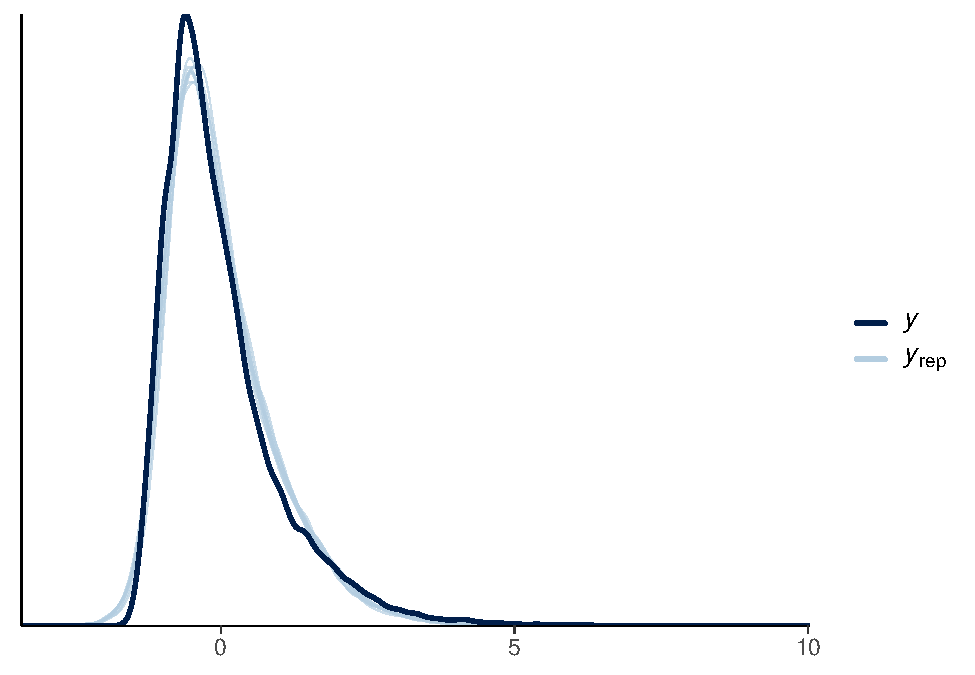
\includegraphics{20_variational_inference_files/figure-latex/Model with block as factor-1.pdf}

\begin{Shaded}
\begin{Highlighting}[]
\NormalTok{m3 }\OtherTok{\textless{}{-}} \FunctionTok{brm}\NormalTok{(}
  \FunctionTok{bf}\NormalTok{(zrt }\SpecialCharTok{\textasciitilde{}}\NormalTok{ CT }\SpecialCharTok{*}\NormalTok{ SC }\SpecialCharTok{*}\NormalTok{ BL }\SpecialCharTok{+}
\NormalTok{       (}\DecValTok{1} \SpecialCharTok{+}\NormalTok{ CT }\SpecialCharTok{*}\NormalTok{ SC }\SpecialCharTok{*}\NormalTok{ BL }\SpecialCharTok{|}\NormalTok{ subj\_id) }\SpecialCharTok{+}\NormalTok{ (}\DecValTok{1} \SpecialCharTok{|}\NormalTok{ movie\_id)}
\NormalTok{  ), }
  \AttributeTok{algorithm =} \StringTok{"meanfield"}\NormalTok{,}
  \AttributeTok{family =} \FunctionTok{asym\_laplace}\NormalTok{(),}
  \AttributeTok{iter =} \DecValTok{20000}\NormalTok{, }\CommentTok{\# Increase the number of iterations}
  \AttributeTok{init =} \FloatTok{0.01}\NormalTok{,}
  \AttributeTok{data =}\NormalTok{ d}
\NormalTok{)}
\end{Highlighting}
\end{Shaded}

\begin{verbatim}
## Compiling Stan program...
\end{verbatim}

\begin{verbatim}
## Trying to compile a simple C file
\end{verbatim}

\begin{verbatim}
## Running /Library/Frameworks/R.framework/Resources/bin/R CMD SHLIB foo.c
## using C compiler: ‘Apple clang version 14.0.3 (clang-1403.0.22.14.1)’
## using SDK: ‘MacOSX13.3.sdk’
## clang -arch arm64 -I"/Library/Frameworks/R.framework/Resources/include" -DNDEBUG   -I"/Library/Frameworks/R.framework/Versions/4.3-arm64/Resources/library/Rcpp/include/"  -I"/Library/Frameworks/R.framework/Versions/4.3-arm64/Resources/library/RcppEigen/include/"  -I"/Library/Frameworks/R.framework/Versions/4.3-arm64/Resources/library/RcppEigen/include/unsupported"  -I"/Library/Frameworks/R.framework/Versions/4.3-arm64/Resources/library/BH/include" -I"/Library/Frameworks/R.framework/Versions/4.3-arm64/Resources/library/StanHeaders/include/src/"  -I"/Library/Frameworks/R.framework/Versions/4.3-arm64/Resources/library/StanHeaders/include/"  -I"/Library/Frameworks/R.framework/Versions/4.3-arm64/Resources/library/RcppParallel/include/"  -I"/Library/Frameworks/R.framework/Versions/4.3-arm64/Resources/library/rstan/include" -DEIGEN_NO_DEBUG  -DBOOST_DISABLE_ASSERTS  -DBOOST_PENDING_INTEGER_LOG2_HPP  -DSTAN_THREADS  -DUSE_STANC3 -DSTRICT_R_HEADERS  -DBOOST_PHOENIX_NO_VARIADIC_EXPRESSION  -DBOOST_NO_AUTO_PTR  -include '/Library/Frameworks/R.framework/Versions/4.3-arm64/Resources/library/StanHeaders/include/stan/math/prim/fun/Eigen.hpp'  -D_REENTRANT -DRCPP_PARALLEL_USE_TBB=1   -I/opt/R/arm64/include    -fPIC  -falign-functions=64 -Wall -g -O2  -c foo.c -o foo.o
## In file included from <built-in>:1:
## In file included from /Library/Frameworks/R.framework/Versions/4.3-arm64/Resources/library/StanHeaders/include/stan/math/prim/fun/Eigen.hpp:22:
## In file included from /Library/Frameworks/R.framework/Versions/4.3-arm64/Resources/library/RcppEigen/include/Eigen/Dense:1:
## In file included from /Library/Frameworks/R.framework/Versions/4.3-arm64/Resources/library/RcppEigen/include/Eigen/Core:88:
## /Library/Frameworks/R.framework/Versions/4.3-arm64/Resources/library/RcppEigen/include/Eigen/src/Core/util/Macros.h:628:1: error: unknown type name 'namespace'
## namespace Eigen {
## ^
## /Library/Frameworks/R.framework/Versions/4.3-arm64/Resources/library/RcppEigen/include/Eigen/src/Core/util/Macros.h:628:16: error: expected ';' after top level declarator
## namespace Eigen {
##                ^
##                ;
## In file included from <built-in>:1:
## In file included from /Library/Frameworks/R.framework/Versions/4.3-arm64/Resources/library/StanHeaders/include/stan/math/prim/fun/Eigen.hpp:22:
## In file included from /Library/Frameworks/R.framework/Versions/4.3-arm64/Resources/library/RcppEigen/include/Eigen/Dense:1:
## /Library/Frameworks/R.framework/Versions/4.3-arm64/Resources/library/RcppEigen/include/Eigen/Core:96:10: fatal error: 'complex' file not found
## #include <complex>
##          ^~~~~~~~~
## 3 errors generated.
## make: *** [foo.o] Error 1
\end{verbatim}

\begin{verbatim}
## Start sampling
\end{verbatim}

\begin{verbatim}
## Chain 1: ------------------------------------------------------------
## Chain 1: EXPERIMENTAL ALGORITHM:
## Chain 1:   This procedure has not been thoroughly tested and may be unstable
## Chain 1:   or buggy. The interface is subject to change.
## Chain 1: ------------------------------------------------------------
## Chain 1: 
## Chain 1: 
## Chain 1: 
## Chain 1: Gradient evaluation took 0.01595 seconds
## Chain 1: 1000 transitions using 10 leapfrog steps per transition would take 159.5 seconds.
## Chain 1: Adjust your expectations accordingly!
## Chain 1: 
## Chain 1: 
## Chain 1: Begin eta adaptation.
## Chain 1: Iteration:   1 / 250 [  0%]  (Adaptation)
## Chain 1: Iteration:  50 / 250 [ 20%]  (Adaptation)
## Chain 1: Iteration: 100 / 250 [ 40%]  (Adaptation)
## Chain 1: Iteration: 150 / 250 [ 60%]  (Adaptation)
## Chain 1: Iteration: 200 / 250 [ 80%]  (Adaptation)
## Chain 1: Iteration: 250 / 250 [100%]  (Adaptation)
## Chain 1: Success! Found best value [eta = 0.1].
## Chain 1: 
## Chain 1: Begin stochastic gradient ascent.
## Chain 1:   iter             ELBO   delta_ELBO_mean   delta_ELBO_med   notes 
## Chain 1:    100       -89242.372             1.000            1.000
## Chain 1:    200       -69762.930             0.640            1.000
## Chain 1:    300       -59435.485             0.484            0.279
## Chain 1:    400       -52369.742             0.397            0.279
## Chain 1:    500       -47080.961             0.340            0.174
## Chain 1:    600       -44839.808             0.292            0.174
## Chain 1:    700       -42276.676             0.259            0.135
## Chain 1:    800       -40885.306             0.231            0.135
## Chain 1:    900       -39443.867             0.209            0.112
## Chain 1:   1000       -38534.916             0.191            0.112
## Chain 1:   1100       -37962.628             0.175            0.061
## Chain 1:   1200       -36940.742             0.162            0.061
## Chain 1:   1300       -36521.419             0.151            0.050
## Chain 1:   1400       -36020.410             0.141            0.050
## Chain 1:   1500       -35625.508             0.132            0.037
## Chain 1:   1600       -35322.309             0.125            0.037
## Chain 1:   1700       -35285.399             0.117            0.034
## Chain 1:   1800       -34956.527             0.111            0.034
## Chain 1:   1900       -34710.912             0.106            0.028
## Chain 1:   2000       -34530.643             0.101            0.028
## Chain 1:   2100       -34466.292             0.051            0.024
## Chain 1:   2200       -34341.981             0.037            0.015
## Chain 1:   2300       -34272.140             0.029            0.014
## Chain 1:   2400       -34198.874             0.022            0.011
## Chain 1:   2500       -34117.966             0.016            0.011
## Chain 1:   2600       -34061.827             0.014            0.009   MEDIAN ELBO CONVERGED
## Chain 1: 
## Chain 1: Drawing a sample of size 1000 from the approximate posterior... 
## Chain 1: COMPLETED.
\end{verbatim}

\begin{verbatim}
## Warning: Pareto k diagnostic value is 13.53. Resampling is disabled. Decreasing
## tol_rel_obj may help if variational algorithm has terminated prematurely.
## Otherwise consider using sampling instead.
\end{verbatim}

\begin{Shaded}
\begin{Highlighting}[]
\NormalTok{loo\_m3 }\OtherTok{\textless{}{-}} \FunctionTok{loo}\NormalTok{(m3)}

\NormalTok{comp }\OtherTok{\textless{}{-}} \FunctionTok{loo\_compare}\NormalTok{(loo\_m3, loo\_m2)}
\FunctionTok{print}\NormalTok{(comp, }\AttributeTok{digits =} \DecValTok{2}\NormalTok{)}
\end{Highlighting}
\end{Shaded}

\begin{verbatim}
##    elpd_diff se_diff
## m2    0.00      0.00
## m3 -738.09     48.10
\end{verbatim}

\begin{Shaded}
\begin{Highlighting}[]
\FunctionTok{pp\_check}\NormalTok{(m3)}
\end{Highlighting}
\end{Shaded}

\begin{verbatim}
## Using 10 posterior draws for ppc type 'dens_overlay' by default.
\end{verbatim}

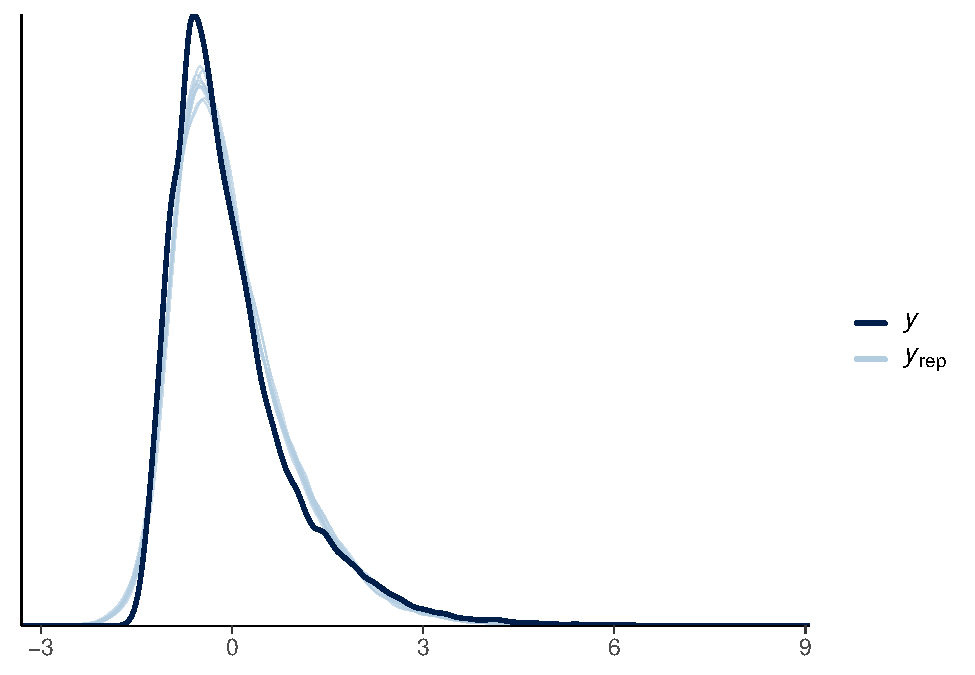
\includegraphics{20_variational_inference_files/figure-latex/Model with block as numeric-1.pdf}

\begin{Shaded}
\begin{Highlighting}[]
\FunctionTok{print}\NormalTok{(loo\_m3)}
\end{Highlighting}
\end{Shaded}

\begin{verbatim}
## 
## Computed from 1000 by 36032 log-likelihood matrix
## 
##          Estimate    SE
## elpd_loo -33846.8 190.3
## p_loo       932.3   6.2
## looic     67693.6 380.6
## ------
## Monte Carlo SE of elpd_loo is 1.0.
## 
## Pareto k diagnostic values:
##                          Count Pct.    Min. n_eff
## (-Inf, 0.5]   (good)     36025 100.0%  524       
##  (0.5, 0.7]   (ok)           7   0.0%  551       
##    (0.7, 1]   (bad)          0   0.0%  <NA>      
##    (1, Inf)   (very bad)     0   0.0%  <NA>      
## 
## All Pareto k estimates are ok (k < 0.7).
## See help('pareto-k-diagnostic') for details.
\end{verbatim}

\begin{Shaded}
\begin{Highlighting}[]
\CommentTok{\# Test whether the kind of video is important within the surprise experiment.}

\NormalTok{m4 }\OtherTok{\textless{}{-}} \FunctionTok{brm}\NormalTok{(}
  \FunctionTok{bf}\NormalTok{(zrt }\SpecialCharTok{\textasciitilde{}}\NormalTok{ CT }\SpecialCharTok{*}\NormalTok{ BL }\SpecialCharTok{+}
\NormalTok{       (}\DecValTok{1} \SpecialCharTok{+}\NormalTok{ CT }\SpecialCharTok{*}\NormalTok{ BL }\SpecialCharTok{|}\NormalTok{ subj\_id) }\SpecialCharTok{+}\NormalTok{ (}\DecValTok{1} \SpecialCharTok{|}\NormalTok{ movie\_id)}
\NormalTok{  ), }
  \AttributeTok{algorithm =} \StringTok{"meanfield"}\NormalTok{,}
  \AttributeTok{family =} \FunctionTok{asym\_laplace}\NormalTok{(),}
  \AttributeTok{iter =} \DecValTok{20000}\NormalTok{, }\CommentTok{\# Increase the number of iterations}
  \AttributeTok{init =} \FloatTok{0.01}\NormalTok{,}
  \AttributeTok{data =}\NormalTok{ d}
\NormalTok{)}
\end{Highlighting}
\end{Shaded}

\begin{verbatim}
## Compiling Stan program...
\end{verbatim}

\begin{verbatim}
## Trying to compile a simple C file
\end{verbatim}

\begin{verbatim}
## Running /Library/Frameworks/R.framework/Resources/bin/R CMD SHLIB foo.c
## using C compiler: ‘Apple clang version 14.0.3 (clang-1403.0.22.14.1)’
## using SDK: ‘MacOSX13.3.sdk’
## clang -arch arm64 -I"/Library/Frameworks/R.framework/Resources/include" -DNDEBUG   -I"/Library/Frameworks/R.framework/Versions/4.3-arm64/Resources/library/Rcpp/include/"  -I"/Library/Frameworks/R.framework/Versions/4.3-arm64/Resources/library/RcppEigen/include/"  -I"/Library/Frameworks/R.framework/Versions/4.3-arm64/Resources/library/RcppEigen/include/unsupported"  -I"/Library/Frameworks/R.framework/Versions/4.3-arm64/Resources/library/BH/include" -I"/Library/Frameworks/R.framework/Versions/4.3-arm64/Resources/library/StanHeaders/include/src/"  -I"/Library/Frameworks/R.framework/Versions/4.3-arm64/Resources/library/StanHeaders/include/"  -I"/Library/Frameworks/R.framework/Versions/4.3-arm64/Resources/library/RcppParallel/include/"  -I"/Library/Frameworks/R.framework/Versions/4.3-arm64/Resources/library/rstan/include" -DEIGEN_NO_DEBUG  -DBOOST_DISABLE_ASSERTS  -DBOOST_PENDING_INTEGER_LOG2_HPP  -DSTAN_THREADS  -DUSE_STANC3 -DSTRICT_R_HEADERS  -DBOOST_PHOENIX_NO_VARIADIC_EXPRESSION  -DBOOST_NO_AUTO_PTR  -include '/Library/Frameworks/R.framework/Versions/4.3-arm64/Resources/library/StanHeaders/include/stan/math/prim/fun/Eigen.hpp'  -D_REENTRANT -DRCPP_PARALLEL_USE_TBB=1   -I/opt/R/arm64/include    -fPIC  -falign-functions=64 -Wall -g -O2  -c foo.c -o foo.o
## In file included from <built-in>:1:
## In file included from /Library/Frameworks/R.framework/Versions/4.3-arm64/Resources/library/StanHeaders/include/stan/math/prim/fun/Eigen.hpp:22:
## In file included from /Library/Frameworks/R.framework/Versions/4.3-arm64/Resources/library/RcppEigen/include/Eigen/Dense:1:
## In file included from /Library/Frameworks/R.framework/Versions/4.3-arm64/Resources/library/RcppEigen/include/Eigen/Core:88:
## /Library/Frameworks/R.framework/Versions/4.3-arm64/Resources/library/RcppEigen/include/Eigen/src/Core/util/Macros.h:628:1: error: unknown type name 'namespace'
## namespace Eigen {
## ^
## /Library/Frameworks/R.framework/Versions/4.3-arm64/Resources/library/RcppEigen/include/Eigen/src/Core/util/Macros.h:628:16: error: expected ';' after top level declarator
## namespace Eigen {
##                ^
##                ;
## In file included from <built-in>:1:
## In file included from /Library/Frameworks/R.framework/Versions/4.3-arm64/Resources/library/StanHeaders/include/stan/math/prim/fun/Eigen.hpp:22:
## In file included from /Library/Frameworks/R.framework/Versions/4.3-arm64/Resources/library/RcppEigen/include/Eigen/Dense:1:
## /Library/Frameworks/R.framework/Versions/4.3-arm64/Resources/library/RcppEigen/include/Eigen/Core:96:10: fatal error: 'complex' file not found
## #include <complex>
##          ^~~~~~~~~
## 3 errors generated.
## make: *** [foo.o] Error 1
\end{verbatim}

\begin{verbatim}
## Start sampling
\end{verbatim}

\begin{verbatim}
## Chain 1: ------------------------------------------------------------
## Chain 1: EXPERIMENTAL ALGORITHM:
## Chain 1:   This procedure has not been thoroughly tested and may be unstable
## Chain 1:   or buggy. The interface is subject to change.
## Chain 1: ------------------------------------------------------------
## Chain 1: 
## Chain 1: 
## Chain 1: 
## Chain 1: Gradient evaluation took 0.012266 seconds
## Chain 1: 1000 transitions using 10 leapfrog steps per transition would take 122.66 seconds.
## Chain 1: Adjust your expectations accordingly!
## Chain 1: 
## Chain 1: 
## Chain 1: Begin eta adaptation.
## Chain 1: Iteration:   1 / 250 [  0%]  (Adaptation)
## Chain 1: Iteration:  50 / 250 [ 20%]  (Adaptation)
## Chain 1: Iteration: 100 / 250 [ 40%]  (Adaptation)
## Chain 1: Iteration: 150 / 250 [ 60%]  (Adaptation)
## Chain 1: Iteration: 200 / 250 [ 80%]  (Adaptation)
## Chain 1: Success! Found best value [eta = 1] earlier than expected.
## Chain 1: 
## Chain 1: Begin stochastic gradient ascent.
## Chain 1:   iter             ELBO   delta_ELBO_mean   delta_ELBO_med   notes 
## Chain 1:    100       -40570.431             1.000            1.000
## Chain 1:    200       -34800.329             0.583            1.000
## Chain 1:    300       -34610.230             0.390            0.166
## Chain 1:    400       -33765.720             0.299            0.166
## Chain 1:    500       -34145.628             0.241            0.025
## Chain 1:    600       -33967.189             0.202            0.025
## Chain 1:    700       -33555.053             0.175            0.012
## Chain 1:    800       -33882.057             0.154            0.012
## Chain 1:    900       -33524.302             0.138            0.011
## Chain 1:   1000       -33239.053             0.125            0.011
## Chain 1:   1100       -33588.039             0.115            0.011
## Chain 1:   1200       -33403.783             0.106            0.011
## Chain 1:   1300       -33480.677             0.098            0.010
## Chain 1:   1400       -33341.290             0.091            0.010
## Chain 1:   1500       -33198.028             0.085            0.010   MEDIAN ELBO CONVERGED
## Chain 1: 
## Chain 1: Drawing a sample of size 1000 from the approximate posterior... 
## Chain 1: COMPLETED.
\end{verbatim}

\begin{verbatim}
## Warning: Pareto k diagnostic value is 7.23. Resampling is disabled. Decreasing
## tol_rel_obj may help if variational algorithm has terminated prematurely.
## Otherwise consider using sampling instead.
\end{verbatim}

\begin{Shaded}
\begin{Highlighting}[]
\NormalTok{loo\_m4 }\OtherTok{\textless{}{-}} \FunctionTok{loo}\NormalTok{(m4)}


\NormalTok{comp }\OtherTok{\textless{}{-}} \FunctionTok{loo\_compare}\NormalTok{(loo\_m3, loo\_m4)}
\FunctionTok{print}\NormalTok{(comp, }\AttributeTok{digits =} \DecValTok{2}\NormalTok{)}
\end{Highlighting}
\end{Shaded}

\begin{verbatim}
##    elpd_diff se_diff 
## m4     0.00      0.00
## m3 -1212.31     52.57
\end{verbatim}

\begin{Shaded}
\begin{Highlighting}[]
\CommentTok{\# Remove the three{-}way interaction}

\NormalTok{m5 }\OtherTok{\textless{}{-}} \FunctionTok{brm}\NormalTok{(}
  \FunctionTok{bf}\NormalTok{(zrt }\SpecialCharTok{\textasciitilde{}}\NormalTok{ CT }\SpecialCharTok{*}\NormalTok{ SC }\SpecialCharTok{+}\NormalTok{ CT }\SpecialCharTok{*}\NormalTok{ BL }\SpecialCharTok{+}\NormalTok{ SC }\SpecialCharTok{*}\NormalTok{ BL }\SpecialCharTok{+} 
\NormalTok{       (}\DecValTok{1} \SpecialCharTok{+}\NormalTok{ CT }\SpecialCharTok{*}\NormalTok{ SC }\SpecialCharTok{+}\NormalTok{ CT }\SpecialCharTok{*}\NormalTok{ BL }\SpecialCharTok{+}\NormalTok{ SC }\SpecialCharTok{*}\NormalTok{ BL }\SpecialCharTok{|}\NormalTok{ subj\_id) }\SpecialCharTok{+}\NormalTok{ (}\DecValTok{1} \SpecialCharTok{|}\NormalTok{ movie\_id)}
\NormalTok{  ), }
  \AttributeTok{algorithm =} \StringTok{"meanfield"}\NormalTok{,}
  \AttributeTok{family =}\NormalTok{ brms}\SpecialCharTok{::}\FunctionTok{asym\_laplace}\NormalTok{(),}
  \AttributeTok{iter =} \DecValTok{20000}\NormalTok{, }\CommentTok{\# Increase the number of iterations}
  \AttributeTok{init =} \FloatTok{0.01}\NormalTok{,}
  \AttributeTok{data =}\NormalTok{ d}
\NormalTok{)}
\end{Highlighting}
\end{Shaded}

\begin{verbatim}
## Compiling Stan program...
\end{verbatim}

\begin{verbatim}
## Trying to compile a simple C file
\end{verbatim}

\begin{verbatim}
## Running /Library/Frameworks/R.framework/Resources/bin/R CMD SHLIB foo.c
## using C compiler: ‘Apple clang version 14.0.3 (clang-1403.0.22.14.1)’
## using SDK: ‘MacOSX13.3.sdk’
## clang -arch arm64 -I"/Library/Frameworks/R.framework/Resources/include" -DNDEBUG   -I"/Library/Frameworks/R.framework/Versions/4.3-arm64/Resources/library/Rcpp/include/"  -I"/Library/Frameworks/R.framework/Versions/4.3-arm64/Resources/library/RcppEigen/include/"  -I"/Library/Frameworks/R.framework/Versions/4.3-arm64/Resources/library/RcppEigen/include/unsupported"  -I"/Library/Frameworks/R.framework/Versions/4.3-arm64/Resources/library/BH/include" -I"/Library/Frameworks/R.framework/Versions/4.3-arm64/Resources/library/StanHeaders/include/src/"  -I"/Library/Frameworks/R.framework/Versions/4.3-arm64/Resources/library/StanHeaders/include/"  -I"/Library/Frameworks/R.framework/Versions/4.3-arm64/Resources/library/RcppParallel/include/"  -I"/Library/Frameworks/R.framework/Versions/4.3-arm64/Resources/library/rstan/include" -DEIGEN_NO_DEBUG  -DBOOST_DISABLE_ASSERTS  -DBOOST_PENDING_INTEGER_LOG2_HPP  -DSTAN_THREADS  -DUSE_STANC3 -DSTRICT_R_HEADERS  -DBOOST_PHOENIX_NO_VARIADIC_EXPRESSION  -DBOOST_NO_AUTO_PTR  -include '/Library/Frameworks/R.framework/Versions/4.3-arm64/Resources/library/StanHeaders/include/stan/math/prim/fun/Eigen.hpp'  -D_REENTRANT -DRCPP_PARALLEL_USE_TBB=1   -I/opt/R/arm64/include    -fPIC  -falign-functions=64 -Wall -g -O2  -c foo.c -o foo.o
## In file included from <built-in>:1:
## In file included from /Library/Frameworks/R.framework/Versions/4.3-arm64/Resources/library/StanHeaders/include/stan/math/prim/fun/Eigen.hpp:22:
## In file included from /Library/Frameworks/R.framework/Versions/4.3-arm64/Resources/library/RcppEigen/include/Eigen/Dense:1:
## In file included from /Library/Frameworks/R.framework/Versions/4.3-arm64/Resources/library/RcppEigen/include/Eigen/Core:88:
## /Library/Frameworks/R.framework/Versions/4.3-arm64/Resources/library/RcppEigen/include/Eigen/src/Core/util/Macros.h:628:1: error: unknown type name 'namespace'
## namespace Eigen {
## ^
## /Library/Frameworks/R.framework/Versions/4.3-arm64/Resources/library/RcppEigen/include/Eigen/src/Core/util/Macros.h:628:16: error: expected ';' after top level declarator
## namespace Eigen {
##                ^
##                ;
## In file included from <built-in>:1:
## In file included from /Library/Frameworks/R.framework/Versions/4.3-arm64/Resources/library/StanHeaders/include/stan/math/prim/fun/Eigen.hpp:22:
## In file included from /Library/Frameworks/R.framework/Versions/4.3-arm64/Resources/library/RcppEigen/include/Eigen/Dense:1:
## /Library/Frameworks/R.framework/Versions/4.3-arm64/Resources/library/RcppEigen/include/Eigen/Core:96:10: fatal error: 'complex' file not found
## #include <complex>
##          ^~~~~~~~~
## 3 errors generated.
## make: *** [foo.o] Error 1
\end{verbatim}

\begin{verbatim}
## Start sampling
\end{verbatim}

\begin{verbatim}
## Chain 1: ------------------------------------------------------------
## Chain 1: EXPERIMENTAL ALGORITHM:
## Chain 1:   This procedure has not been thoroughly tested and may be unstable
## Chain 1:   or buggy. The interface is subject to change.
## Chain 1: ------------------------------------------------------------
## Chain 1: 
## Chain 1: 
## Chain 1: 
## Chain 1: Gradient evaluation took 0.014241 seconds
## Chain 1: 1000 transitions using 10 leapfrog steps per transition would take 142.41 seconds.
## Chain 1: Adjust your expectations accordingly!
## Chain 1: 
## Chain 1: 
## Chain 1: Begin eta adaptation.
## Chain 1: Iteration:   1 / 250 [  0%]  (Adaptation)
## Chain 1: Iteration:  50 / 250 [ 20%]  (Adaptation)
## Chain 1: Iteration: 100 / 250 [ 40%]  (Adaptation)
## Chain 1: Iteration: 150 / 250 [ 60%]  (Adaptation)
## Chain 1: Iteration: 200 / 250 [ 80%]  (Adaptation)
## Chain 1: Iteration: 250 / 250 [100%]  (Adaptation)
## Chain 1: Success! Found best value [eta = 0.1].
## Chain 1: 
## Chain 1: Begin stochastic gradient ascent.
## Chain 1:   iter             ELBO   delta_ELBO_mean   delta_ELBO_med   notes 
## Chain 1:    100      -207014.447             1.000            1.000
## Chain 1:    200      -122442.623             0.845            1.000
## Chain 1:    300       -98153.633             0.646            0.691
## Chain 1:    400       -83033.265             0.530            0.691
## Chain 1:    500       -71462.777             0.456            0.247
## Chain 1:    600       -63569.721             0.401            0.247
## Chain 1:    700       -57622.000             0.359            0.182
## Chain 1:    800       -53208.407             0.324            0.182
## Chain 1:    900       -50186.756             0.295            0.162
## Chain 1:   1000       -48587.525             0.269            0.162
## Chain 1:   1100       -45945.649             0.249            0.124
## Chain 1:   1200       -44571.188             0.231            0.124
## Chain 1:   1300       -43124.783             0.216            0.103
## Chain 1:   1400       -42257.253             0.202            0.103
## Chain 1:   1500       -41121.245             0.190            0.083
## Chain 1:   1600       -40378.575             0.180            0.083
## Chain 1:   1700       -39909.204             0.170            0.060
## Chain 1:   1800       -39233.737             0.161            0.060
## Chain 1:   1900       -38708.476             0.154            0.058
## Chain 1:   2000       -38414.435             0.146            0.058
## Chain 1:   2100       -38064.603             0.097            0.034
## Chain 1:   2200       -37716.130             0.063            0.033
## Chain 1:   2300       -37522.596             0.050            0.031
## Chain 1:   2400       -37267.549             0.042            0.028
## Chain 1:   2500       -36987.929             0.034            0.021
## Chain 1:   2600       -36934.083             0.028            0.018
## Chain 1:   2700       -36714.540             0.023            0.017
## Chain 1:   2800       -36588.581             0.019            0.014
## Chain 1:   2900       -36478.459             0.016            0.012
## Chain 1:   3000       -36375.133             0.015            0.009   MEDIAN ELBO CONVERGED
## Chain 1: 
## Chain 1: Drawing a sample of size 1000 from the approximate posterior... 
## Chain 1: COMPLETED.
\end{verbatim}

\begin{verbatim}
## Warning: Pareto k diagnostic value is 25.03. Resampling is disabled. Decreasing
## tol_rel_obj may help if variational algorithm has terminated prematurely.
## Otherwise consider using sampling instead.
\end{verbatim}

\begin{Shaded}
\begin{Highlighting}[]
\NormalTok{loo\_m5 }\OtherTok{\textless{}{-}} \FunctionTok{loo}\NormalTok{(m5)}

\CommentTok{\# Test of the three{-}way interaction}
\NormalTok{comp }\OtherTok{\textless{}{-}} \FunctionTok{loo\_compare}\NormalTok{(loo\_m3, loo\_m5)}
\FunctionTok{print}\NormalTok{(comp, }\AttributeTok{digits =} \DecValTok{2}\NormalTok{)}
\end{Highlighting}
\end{Shaded}

\begin{verbatim}
##    elpd_diff se_diff 
## m3     0.00      0.00
## m5 -2405.31     80.41
\end{verbatim}

\begin{Shaded}
\begin{Highlighting}[]
\CommentTok{\# Conditional plot.}

\NormalTok{mod }\OtherTok{\textless{}{-}}\NormalTok{ m3}

\CommentTok{\# Three{-}way interaction}
\NormalTok{conditions }\OtherTok{\textless{}{-}} \FunctionTok{make\_conditions}\NormalTok{(mod, }\StringTok{"SC"}\NormalTok{)}
\NormalTok{c\_eff }\OtherTok{\textless{}{-}} \FunctionTok{conditional\_effects}\NormalTok{(mod, }\StringTok{"BL:CT"}\NormalTok{, }\AttributeTok{conditions=}\NormalTok{conditions) }
\FunctionTok{plot}\NormalTok{(c\_eff, }\AttributeTok{plot =} \ConstantTok{FALSE}\NormalTok{)[[}\DecValTok{1}\NormalTok{]] }\SpecialCharTok{+}
  \FunctionTok{theme}\NormalTok{(}\AttributeTok{legend.position =} \StringTok{"bottom"}\NormalTok{) }\SpecialCharTok{+}
  \FunctionTok{labs}\NormalTok{(}
    \AttributeTok{y =} \StringTok{"Reaction Times (standardized)"}\NormalTok{,}
    \AttributeTok{x =} \StringTok{"Block of Trials"}
\NormalTok{  )}
\end{Highlighting}
\end{Shaded}

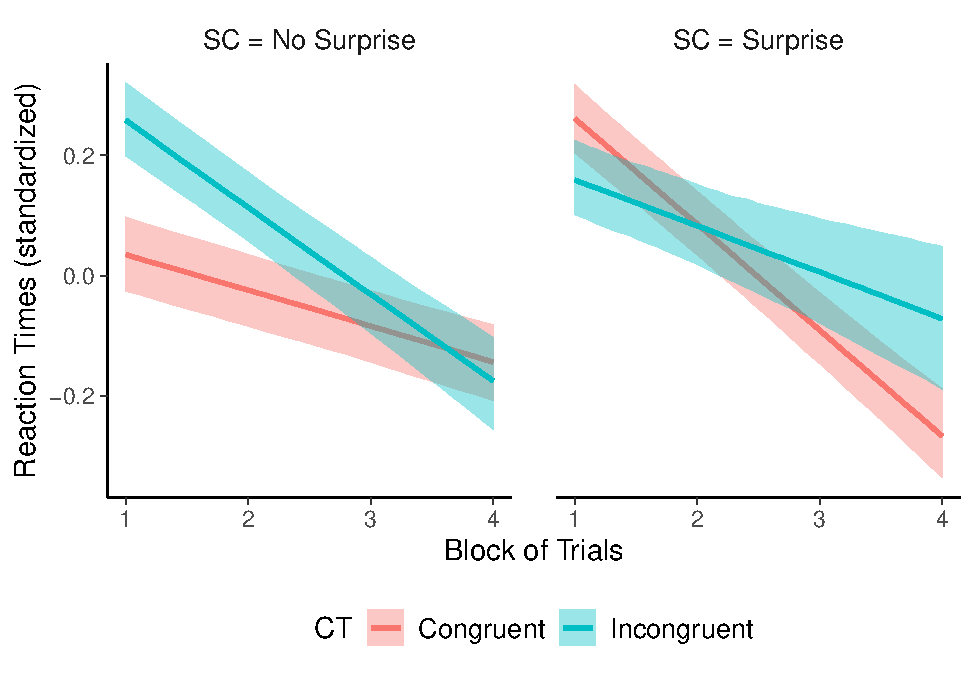
\includegraphics{20_variational_inference_files/figure-latex/unnamed-chunk-16-1.pdf}

\begin{Shaded}
\begin{Highlighting}[]
\CommentTok{\# Plot of the raw data means}

\FunctionTok{plot}\NormalTok{(}\FunctionTok{density}\NormalTok{(}\FunctionTok{log}\NormalTok{(surprise\_cor\_df}\SpecialCharTok{$}\NormalTok{rt)))}
\end{Highlighting}
\end{Shaded}

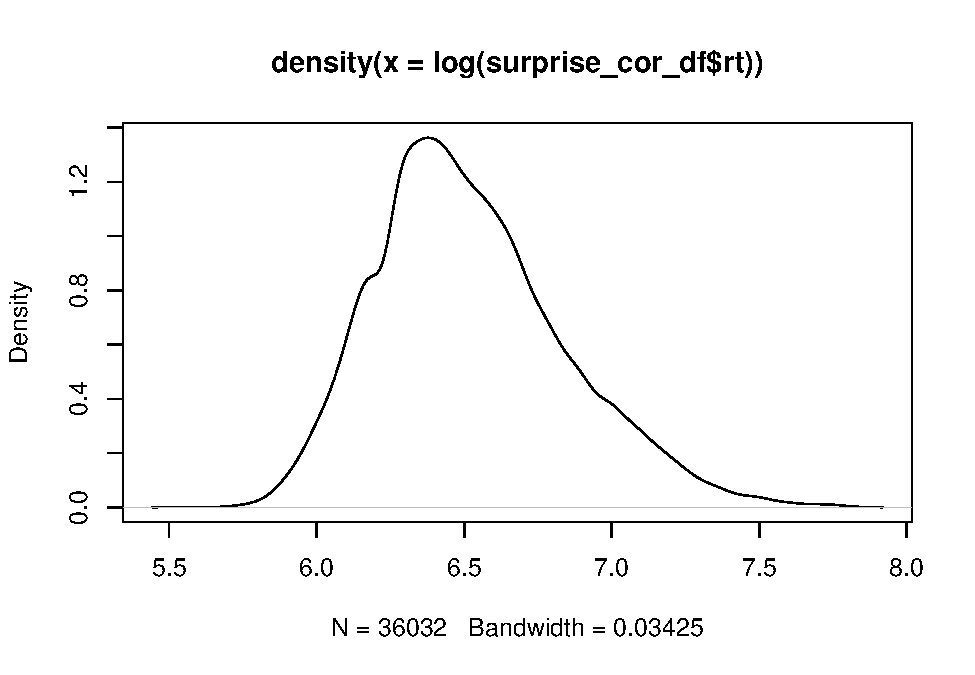
\includegraphics{20_variational_inference_files/figure-latex/unnamed-chunk-17-1.pdf}

\begin{Shaded}
\begin{Highlighting}[]
\NormalTok{surprise\_cor\_df}\SpecialCharTok{$}\NormalTok{lrt }\OtherTok{\textless{}{-}} \FunctionTok{log}\NormalTok{(surprise\_cor\_df}\SpecialCharTok{$}\NormalTok{rt)}

\CommentTok{\# Calculate the within{-}subject mean and standard error for each condition}
\NormalTok{subject\_summary }\OtherTok{\textless{}{-}}\NormalTok{ surprise\_cor\_df }\SpecialCharTok{\%\textgreater{}\%}
  \FunctionTok{group\_by}\NormalTok{(subj\_id, SC, CT, BL) }\SpecialCharTok{\%\textgreater{}\%}
  \FunctionTok{summarize}\NormalTok{(}
    \AttributeTok{subj\_mean =} \FunctionTok{mean}\NormalTok{(lrt, }\AttributeTok{na.rm =} \ConstantTok{TRUE}\NormalTok{),}
    \AttributeTok{.groups =} \StringTok{\textquotesingle{}drop\textquotesingle{}}
\NormalTok{  )}

\CommentTok{\# Calculate the overall mean and within{-}subject standard error for each condition}
\NormalTok{plot\_df }\OtherTok{\textless{}{-}}\NormalTok{ subject\_summary }\SpecialCharTok{\%\textgreater{}\%}
  \FunctionTok{group\_by}\NormalTok{(SC, CT, BL) }\SpecialCharTok{\%\textgreater{}\%}
  \FunctionTok{summarize}\NormalTok{(}
    \AttributeTok{m =} \FunctionTok{mean}\NormalTok{(subj\_mean, }\AttributeTok{na.rm =} \ConstantTok{TRUE}\NormalTok{),}
    \AttributeTok{stderr =} \FunctionTok{sd}\NormalTok{(subj\_mean, }\AttributeTok{na.rm =} \ConstantTok{TRUE}\NormalTok{) }\SpecialCharTok{/} \FunctionTok{sqrt}\NormalTok{(}\FunctionTok{n}\NormalTok{()),}
    \AttributeTok{.groups =} \StringTok{\textquotesingle{}drop\textquotesingle{}}
\NormalTok{  )}

\CommentTok{\# Create the lower and upper bounds for the error bars}
\NormalTok{plot\_df}\SpecialCharTok{$}\NormalTok{lower }\OtherTok{\textless{}{-}}\NormalTok{ plot\_df}\SpecialCharTok{$}\NormalTok{m }\SpecialCharTok{{-}}\NormalTok{ plot\_df}\SpecialCharTok{$}\NormalTok{stderr}
\NormalTok{plot\_df}\SpecialCharTok{$}\NormalTok{upper }\OtherTok{\textless{}{-}}\NormalTok{ plot\_df}\SpecialCharTok{$}\NormalTok{m }\SpecialCharTok{+}\NormalTok{ plot\_df}\SpecialCharTok{$}\NormalTok{stderr}

\NormalTok{plot\_df}\SpecialCharTok{$}\NormalTok{m }\OtherTok{\textless{}{-}} \FunctionTok{exp}\NormalTok{(plot\_df}\SpecialCharTok{$}\NormalTok{m)}
\NormalTok{plot\_df}\SpecialCharTok{$}\NormalTok{stderr }\OtherTok{\textless{}{-}} \FunctionTok{exp}\NormalTok{(plot\_df}\SpecialCharTok{$}\NormalTok{stderr)}
\NormalTok{plot\_df}\SpecialCharTok{$}\NormalTok{lower }\OtherTok{\textless{}{-}} \FunctionTok{exp}\NormalTok{(plot\_df}\SpecialCharTok{$}\NormalTok{lower)}
\NormalTok{plot\_df}\SpecialCharTok{$}\NormalTok{upper }\OtherTok{\textless{}{-}} \FunctionTok{exp}\NormalTok{(plot\_df}\SpecialCharTok{$}\NormalTok{upper)}

\CommentTok{\# Create the plot}
\NormalTok{pd }\OtherTok{\textless{}{-}} \FunctionTok{position\_dodge}\NormalTok{(}\FloatTok{0.5}\NormalTok{)}

\FunctionTok{ggplot}\NormalTok{(plot\_df, }\FunctionTok{aes}\NormalTok{(}\AttributeTok{x =}\NormalTok{ BL, }\AttributeTok{y =}\NormalTok{ m, }\AttributeTok{color =}\NormalTok{ CT)) }\SpecialCharTok{+}
  \FunctionTok{geom\_pointrange}\NormalTok{(}\FunctionTok{aes}\NormalTok{(}\AttributeTok{ymin =}\NormalTok{ lower, }\AttributeTok{ymax =}\NormalTok{ upper), }\AttributeTok{lwd =} \FloatTok{1.05}\NormalTok{, }\AttributeTok{position =}\NormalTok{ pd) }\SpecialCharTok{+}
  \FunctionTok{geom\_line}\NormalTok{(}\AttributeTok{position =}\NormalTok{ pd, }\AttributeTok{lwd =} \FloatTok{1.05}\NormalTok{) }\SpecialCharTok{+}
  \FunctionTok{geom\_point}\NormalTok{(}\AttributeTok{position =}\NormalTok{ pd, }\AttributeTok{size =} \DecValTok{5}\NormalTok{) }\SpecialCharTok{+}
  \FunctionTok{facet\_grid}\NormalTok{(}\SpecialCharTok{\textasciitilde{}}\NormalTok{SC) }\SpecialCharTok{+}
  \FunctionTok{xlab}\NormalTok{(}\StringTok{"Block"}\NormalTok{) }\SpecialCharTok{+}
  \FunctionTok{ylab}\NormalTok{(}\StringTok{"RT (ms)"}\NormalTok{) }\SpecialCharTok{+}
  \FunctionTok{theme}\NormalTok{(}\AttributeTok{legend.position =} \StringTok{"bottom"}\NormalTok{)}
\end{Highlighting}
\end{Shaded}

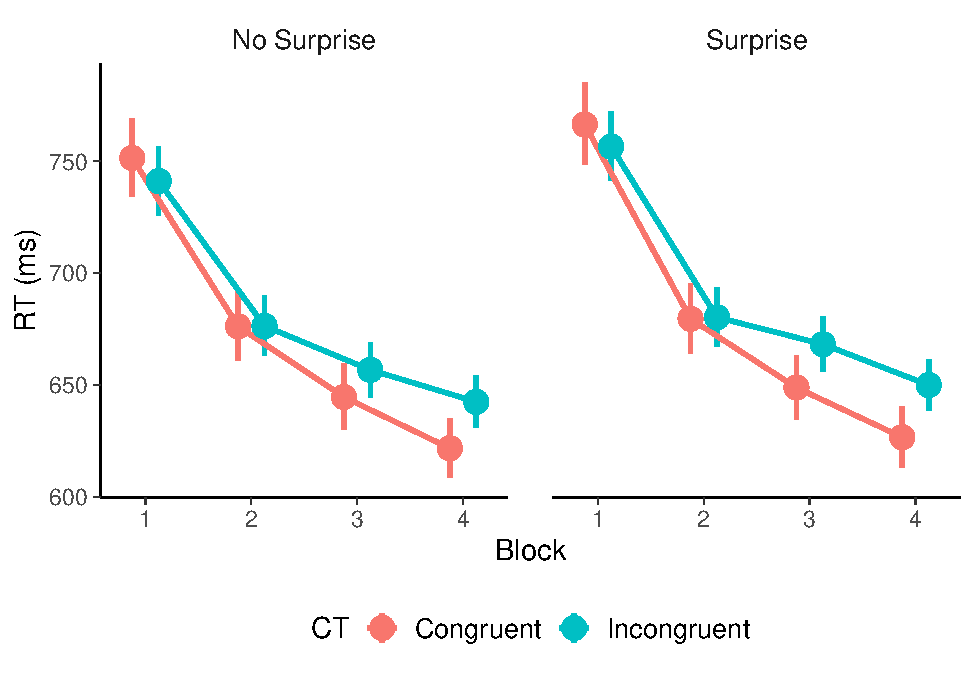
\includegraphics{20_variational_inference_files/figure-latex/unnamed-chunk-17-2.pdf}

\begin{Shaded}
\begin{Highlighting}[]
\CommentTok{\# Compute contrasts.}

\NormalTok{mod }\OtherTok{\textless{}{-}}\NormalTok{ m2  }\CommentTok{\# Use block as factor}

\CommentTok{\#get the adjusted means}
\NormalTok{em }\OtherTok{\textless{}{-}} \FunctionTok{emmeans}\NormalTok{ (mod, }\SpecialCharTok{\textasciitilde{}}\NormalTok{ BF}\SpecialCharTok{:}\NormalTok{CT }\SpecialCharTok{|}\NormalTok{ SC)}
\NormalTok{em}
\end{Highlighting}
\end{Shaded}

\begin{verbatim}
## SC = No Surprise:
##  BF CT             emmean lower.HPD upper.HPD
##  1  Congruent   -0.000897 -0.032312    0.0406
##  2  Congruent   -0.152757 -0.192000   -0.1037
##  3  Congruent   -0.267424 -0.308094   -0.2225
##  4  Congruent   -0.327470 -0.365367   -0.2880
##  1  Incongruent  0.039031  0.000861    0.0746
##  2  Incongruent -0.105621 -0.160468   -0.0412
##  3  Incongruent -0.204678 -0.261306   -0.1553
##  4  Incongruent -0.256855 -0.315761   -0.2029
## 
## SC = Surprise:
##  BF CT             emmean lower.HPD upper.HPD
##  1  Congruent    0.410658  0.375315    0.4449
##  2  Congruent    0.154978  0.103596    0.2113
##  3  Congruent    0.049769  0.000821    0.0988
##  4  Congruent   -0.020332 -0.066870    0.0301
##  1  Incongruent  0.385291  0.348062    0.4273
##  2  Incongruent  0.221274  0.134159    0.3028
##  3  Incongruent  0.139107  0.059979    0.2150
##  4  Incongruent  0.109118  0.028787    0.1885
## 
## Point estimate displayed: median 
## HPD interval probability: 0.95
\end{verbatim}

\begin{Shaded}
\begin{Highlighting}[]
\CommentTok{\#get all possible contrasts}
\NormalTok{cont }\OtherTok{\textless{}{-}} \FunctionTok{contrast}\NormalTok{(em, }\StringTok{"tukey"}\NormalTok{)}
\NormalTok{cont}
\end{Highlighting}
\end{Shaded}

\begin{verbatim}
## SC = No Surprise:
##  contrast                          estimate lower.HPD upper.HPD
##  BF1 Congruent - BF2 Congruent       0.1517   0.11712    0.1873
##  BF1 Congruent - BF3 Congruent       0.2672   0.23908    0.3008
##  BF1 Congruent - BF4 Congruent       0.3271   0.29705    0.3527
##  BF1 Congruent - BF1 Incongruent    -0.0384  -0.06414   -0.0172
##  BF1 Congruent - BF2 Incongruent     0.1047   0.04086    0.1645
##  BF1 Congruent - BF3 Incongruent     0.2048   0.14835    0.2578
##  BF1 Congruent - BF4 Incongruent     0.2583   0.19999    0.3126
##  BF2 Congruent - BF3 Congruent       0.1152   0.06729    0.1615
##  BF2 Congruent - BF4 Congruent       0.1756   0.13128    0.2188
##  BF2 Congruent - BF1 Incongruent    -0.1908  -0.23335   -0.1458
##  BF2 Congruent - BF2 Incongruent    -0.0464  -0.09265    0.0107
##  BF2 Congruent - BF3 Incongruent     0.0537  -0.01071    0.1193
##  BF2 Congruent - BF4 Incongruent     0.1043   0.03420    0.1704
##  BF3 Congruent - BF4 Congruent       0.0588   0.01845    0.0980
##  BF3 Congruent - BF1 Incongruent    -0.3061  -0.34778   -0.2723
##  BF3 Congruent - BF2 Incongruent    -0.1621  -0.23261   -0.0920
##  BF3 Congruent - BF3 Incongruent    -0.0617  -0.10611   -0.0182
##  BF3 Congruent - BF4 Incongruent    -0.0119  -0.06913    0.0529
##  BF4 Congruent - BF1 Incongruent    -0.3653  -0.40390   -0.3315
##  BF4 Congruent - BF2 Incongruent    -0.2204  -0.29316   -0.1582
##  BF4 Congruent - BF3 Incongruent    -0.1224  -0.17890   -0.0609
##  BF4 Congruent - BF4 Incongruent    -0.0697  -0.11884   -0.0240
##  BF1 Incongruent - BF2 Incongruent   0.1438   0.08799    0.2000
##  BF1 Incongruent - BF3 Incongruent   0.2435   0.19492    0.2899
##  BF1 Incongruent - BF4 Incongruent   0.2957   0.24368    0.3449
##  BF2 Incongruent - BF3 Incongruent   0.1013   0.02934    0.1738
##  BF2 Incongruent - BF4 Incongruent   0.1524   0.07600    0.2293
##  BF3 Incongruent - BF4 Incongruent   0.0516  -0.01850    0.1191
## 
## SC = Surprise:
##  contrast                          estimate lower.HPD upper.HPD
##  BF1 Congruent - BF2 Congruent       0.2552   0.20116    0.3061
##  BF1 Congruent - BF3 Congruent       0.3607   0.31800    0.4112
##  BF1 Congruent - BF4 Congruent       0.4308   0.38522    0.4784
##  BF1 Congruent - BF1 Incongruent     0.0244  -0.01648    0.0619
##  BF1 Congruent - BF2 Incongruent     0.1898   0.09369    0.2826
##  BF1 Congruent - BF3 Incongruent     0.2747   0.19121    0.3616
##  BF1 Congruent - BF4 Incongruent     0.3013   0.21352    0.3998
##  BF2 Congruent - BF3 Congruent       0.1047   0.03761    0.1781
##  BF2 Congruent - BF4 Congruent       0.1738   0.10725    0.2468
##  BF2 Congruent - BF1 Incongruent    -0.2302  -0.29010   -0.1587
##  BF2 Congruent - BF2 Incongruent    -0.0681  -0.14027    0.0140
##  BF2 Congruent - BF3 Incongruent     0.0168  -0.08702    0.1098
##  BF2 Congruent - BF4 Incongruent     0.0469  -0.05754    0.1469
##  BF3 Congruent - BF4 Congruent       0.0686   0.00805    0.1367
##  BF3 Congruent - BF1 Incongruent    -0.3365  -0.39746   -0.2790
##  BF3 Congruent - BF2 Incongruent    -0.1722  -0.28552   -0.0772
##  BF3 Congruent - BF3 Incongruent    -0.0893  -0.16195   -0.0213
##  BF3 Congruent - BF4 Incongruent    -0.0593  -0.15902    0.0363
##  BF4 Congruent - BF1 Incongruent    -0.4058  -0.46263   -0.3442
##  BF4 Congruent - BF2 Incongruent    -0.2400  -0.34569   -0.1359
##  BF4 Congruent - BF3 Incongruent    -0.1577  -0.26298   -0.0704
##  BF4 Congruent - BF4 Incongruent    -0.1283  -0.20336   -0.0587
##  BF1 Incongruent - BF2 Incongruent   0.1642   0.07679    0.2521
##  BF1 Incongruent - BF3 Incongruent   0.2489   0.17045    0.3220
##  BF1 Incongruent - BF4 Incongruent   0.2767   0.19663    0.3616
##  BF2 Incongruent - BF3 Incongruent   0.0877  -0.03519    0.1919
##  BF2 Incongruent - BF4 Incongruent   0.1139   0.00548    0.2377
##  BF3 Incongruent - BF4 Incongruent   0.0269  -0.10537    0.1244
## 
## Point estimate displayed: median 
## HPD interval probability: 0.95
\end{verbatim}

\begin{Shaded}
\begin{Highlighting}[]
\CommentTok{\#get the posterior draws from the contrasts}
\NormalTok{cont\_posterior }\OtherTok{\textless{}{-}} \FunctionTok{gather\_emmeans\_draws}\NormalTok{(cont)}

\CommentTok{\#plot}
\FunctionTok{ggplot}\NormalTok{(cont\_posterior,}
       \FunctionTok{aes}\NormalTok{(}\AttributeTok{y =}\NormalTok{ contrast, }\AttributeTok{x =}\NormalTok{ .value)) }\SpecialCharTok{+}
  \FunctionTok{stat\_halfeye}\NormalTok{() }\SpecialCharTok{+}
  \FunctionTok{facet\_wrap}\NormalTok{(}\SpecialCharTok{\textasciitilde{}}\NormalTok{SC) }\SpecialCharTok{+}
  \FunctionTok{geom\_vline}\NormalTok{(}\AttributeTok{xintercept =} \DecValTok{0}\NormalTok{, }\AttributeTok{color =} \StringTok{"red"}\NormalTok{, }\AttributeTok{lty =} \DecValTok{2}\NormalTok{)}
\end{Highlighting}
\end{Shaded}

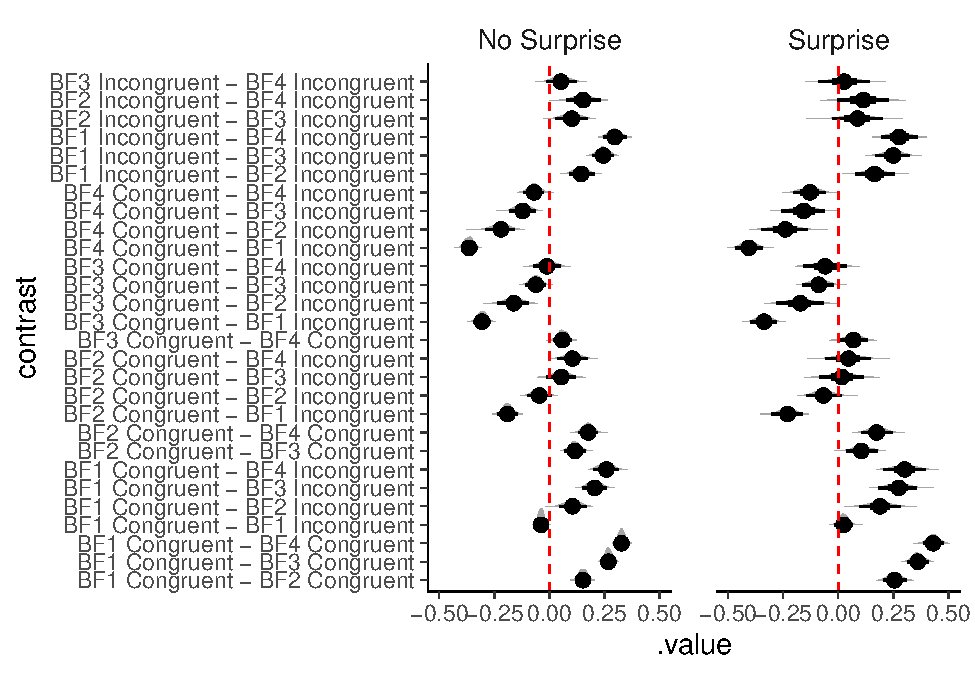
\includegraphics{20_variational_inference_files/figure-latex/unnamed-chunk-18-1.pdf}

\begin{Shaded}
\begin{Highlighting}[]
\CommentTok{\# Control experiment}
\end{Highlighting}
\end{Shaded}

\begin{Shaded}
\begin{Highlighting}[]
\NormalTok{control\_cor\_df}\SpecialCharTok{$}\NormalTok{blk }\OtherTok{\textless{}{-}} \FunctionTok{factor}\NormalTok{(control\_cor\_df}\SpecialCharTok{$}\NormalTok{block)}

\NormalTok{control\_cor\_df}\SpecialCharTok{$}\NormalTok{zrt }\OtherTok{\textless{}{-}} \FunctionTok{scale}\NormalTok{(control\_cor\_df}\SpecialCharTok{$}\NormalTok{rt) }\SpecialCharTok{|\textgreater{}} 
  \FunctionTok{as.numeric}\NormalTok{()}

\NormalTok{control\_cor\_df}\SpecialCharTok{$}\NormalTok{CT }\OtherTok{\textless{}{-}}\NormalTok{ control\_cor\_df}\SpecialCharTok{$}\NormalTok{is\_congruent\_trial }\SpecialCharTok{|\textgreater{}} 
  \FunctionTok{as.factor}\NormalTok{()}

\NormalTok{control\_cor\_df}\SpecialCharTok{$}\NormalTok{BF }\OtherTok{\textless{}{-}}\NormalTok{ control\_cor\_df}\SpecialCharTok{$}\NormalTok{blk}
\NormalTok{control\_cor\_df}\SpecialCharTok{$}\NormalTok{BL }\OtherTok{\textless{}{-}}\NormalTok{ control\_cor\_df}\SpecialCharTok{$}\NormalTok{block}

\NormalTok{control\_cor\_df}\SpecialCharTok{$}\NormalTok{movie\_id }\OtherTok{\textless{}{-}} \FunctionTok{factor}\NormalTok{(control\_cor\_df}\SpecialCharTok{$}\NormalTok{movie\_id)}
\NormalTok{control\_cor\_df}\SpecialCharTok{$}\NormalTok{subj\_id }\OtherTok{\textless{}{-}} \FunctionTok{factor}\NormalTok{(control\_cor\_df}\SpecialCharTok{$}\NormalTok{subj\_id)}


\NormalTok{dc }\OtherTok{\textless{}{-}}\NormalTok{ control\_cor\_df }\SpecialCharTok{|\textgreater{}} 
\NormalTok{  dplyr}\SpecialCharTok{::}\FunctionTok{select}\NormalTok{(zrt, CT, BL, BF, subj\_id, movie\_id) }
\end{Highlighting}
\end{Shaded}

\begin{verbatim}
## Adding missing grouping variables: `subj_name`
\end{verbatim}

\begin{Shaded}
\begin{Highlighting}[]
\NormalTok{c3 }\OtherTok{\textless{}{-}} \FunctionTok{brm}\NormalTok{(}
  \FunctionTok{bf}\NormalTok{(zrt }\SpecialCharTok{\textasciitilde{}}\NormalTok{ CT }\SpecialCharTok{*}\NormalTok{ BL }\SpecialCharTok{+}
\NormalTok{       (}\DecValTok{1} \SpecialCharTok{+}\NormalTok{ CT }\SpecialCharTok{*}\NormalTok{ BL }\SpecialCharTok{|}\NormalTok{ subj\_id) }\SpecialCharTok{+}\NormalTok{ (}\DecValTok{1} \SpecialCharTok{|}\NormalTok{ movie\_id)}
\NormalTok{  ), }
  \AttributeTok{algorithm =} \StringTok{"meanfield"}\NormalTok{,}
  \AttributeTok{family =}\NormalTok{ brms}\SpecialCharTok{::}\FunctionTok{asym\_laplace}\NormalTok{(),}
  \AttributeTok{iter =} \DecValTok{20000}\NormalTok{, }\CommentTok{\# Increase the number of iterations}
  \AttributeTok{init =} \FloatTok{0.01}\NormalTok{,}
  \AttributeTok{data =}\NormalTok{ dc}
\NormalTok{)}
\end{Highlighting}
\end{Shaded}

\begin{verbatim}
## Compiling Stan program...
\end{verbatim}

\begin{verbatim}
## Trying to compile a simple C file
\end{verbatim}

\begin{verbatim}
## Running /Library/Frameworks/R.framework/Resources/bin/R CMD SHLIB foo.c
## using C compiler: ‘Apple clang version 14.0.3 (clang-1403.0.22.14.1)’
## using SDK: ‘MacOSX13.3.sdk’
## clang -arch arm64 -I"/Library/Frameworks/R.framework/Resources/include" -DNDEBUG   -I"/Library/Frameworks/R.framework/Versions/4.3-arm64/Resources/library/Rcpp/include/"  -I"/Library/Frameworks/R.framework/Versions/4.3-arm64/Resources/library/RcppEigen/include/"  -I"/Library/Frameworks/R.framework/Versions/4.3-arm64/Resources/library/RcppEigen/include/unsupported"  -I"/Library/Frameworks/R.framework/Versions/4.3-arm64/Resources/library/BH/include" -I"/Library/Frameworks/R.framework/Versions/4.3-arm64/Resources/library/StanHeaders/include/src/"  -I"/Library/Frameworks/R.framework/Versions/4.3-arm64/Resources/library/StanHeaders/include/"  -I"/Library/Frameworks/R.framework/Versions/4.3-arm64/Resources/library/RcppParallel/include/"  -I"/Library/Frameworks/R.framework/Versions/4.3-arm64/Resources/library/rstan/include" -DEIGEN_NO_DEBUG  -DBOOST_DISABLE_ASSERTS  -DBOOST_PENDING_INTEGER_LOG2_HPP  -DSTAN_THREADS  -DUSE_STANC3 -DSTRICT_R_HEADERS  -DBOOST_PHOENIX_NO_VARIADIC_EXPRESSION  -DBOOST_NO_AUTO_PTR  -include '/Library/Frameworks/R.framework/Versions/4.3-arm64/Resources/library/StanHeaders/include/stan/math/prim/fun/Eigen.hpp'  -D_REENTRANT -DRCPP_PARALLEL_USE_TBB=1   -I/opt/R/arm64/include    -fPIC  -falign-functions=64 -Wall -g -O2  -c foo.c -o foo.o
## In file included from <built-in>:1:
## In file included from /Library/Frameworks/R.framework/Versions/4.3-arm64/Resources/library/StanHeaders/include/stan/math/prim/fun/Eigen.hpp:22:
## In file included from /Library/Frameworks/R.framework/Versions/4.3-arm64/Resources/library/RcppEigen/include/Eigen/Dense:1:
## In file included from /Library/Frameworks/R.framework/Versions/4.3-arm64/Resources/library/RcppEigen/include/Eigen/Core:88:
## /Library/Frameworks/R.framework/Versions/4.3-arm64/Resources/library/RcppEigen/include/Eigen/src/Core/util/Macros.h:628:1: error: unknown type name 'namespace'
## namespace Eigen {
## ^
## /Library/Frameworks/R.framework/Versions/4.3-arm64/Resources/library/RcppEigen/include/Eigen/src/Core/util/Macros.h:628:16: error: expected ';' after top level declarator
## namespace Eigen {
##                ^
##                ;
## In file included from <built-in>:1:
## In file included from /Library/Frameworks/R.framework/Versions/4.3-arm64/Resources/library/StanHeaders/include/stan/math/prim/fun/Eigen.hpp:22:
## In file included from /Library/Frameworks/R.framework/Versions/4.3-arm64/Resources/library/RcppEigen/include/Eigen/Dense:1:
## /Library/Frameworks/R.framework/Versions/4.3-arm64/Resources/library/RcppEigen/include/Eigen/Core:96:10: fatal error: 'complex' file not found
## #include <complex>
##          ^~~~~~~~~
## 3 errors generated.
## make: *** [foo.o] Error 1
\end{verbatim}

\begin{verbatim}
## Start sampling
\end{verbatim}

\begin{verbatim}
## Chain 1: ------------------------------------------------------------
## Chain 1: EXPERIMENTAL ALGORITHM:
## Chain 1:   This procedure has not been thoroughly tested and may be unstable
## Chain 1:   or buggy. The interface is subject to change.
## Chain 1: ------------------------------------------------------------
## Chain 1: 
## Chain 1: 
## Chain 1: 
## Chain 1: Gradient evaluation took 0.008785 seconds
## Chain 1: 1000 transitions using 10 leapfrog steps per transition would take 87.85 seconds.
## Chain 1: Adjust your expectations accordingly!
## Chain 1: 
## Chain 1: 
## Chain 1: Begin eta adaptation.
## Chain 1: Iteration:   1 / 250 [  0%]  (Adaptation)
## Chain 1: Iteration:  50 / 250 [ 20%]  (Adaptation)
## Chain 1: Iteration: 100 / 250 [ 40%]  (Adaptation)
## Chain 1: Iteration: 150 / 250 [ 60%]  (Adaptation)
## Chain 1: Iteration: 200 / 250 [ 80%]  (Adaptation)
## Chain 1: Success! Found best value [eta = 1] earlier than expected.
## Chain 1: 
## Chain 1: Begin stochastic gradient ascent.
## Chain 1:   iter             ELBO   delta_ELBO_mean   delta_ELBO_med   notes 
## Chain 1:    100       -26834.126             1.000            1.000
## Chain 1:    200       -26134.424             0.513            1.000
## Chain 1:    300       -25621.156             0.349            0.027
## Chain 1:    400       -25513.701             0.263            0.027
## Chain 1:    500       -25239.639             0.212            0.020
## Chain 1:    600       -25221.502             0.177            0.020
## Chain 1:    700       -25255.717             0.152            0.011
## Chain 1:    800       -25050.032             0.134            0.011
## Chain 1:    900       -25031.850             0.119            0.008   MEDIAN ELBO CONVERGED
## Chain 1: 
## Chain 1: Drawing a sample of size 1000 from the approximate posterior... 
## Chain 1: COMPLETED.
\end{verbatim}

\begin{verbatim}
## Warning: Pareto k diagnostic value is 7.11. Resampling is disabled. Decreasing
## tol_rel_obj may help if variational algorithm has terminated prematurely.
## Otherwise consider using sampling instead.
\end{verbatim}

\begin{Shaded}
\begin{Highlighting}[]
\NormalTok{loo\_c3 }\OtherTok{\textless{}{-}} \FunctionTok{loo}\NormalTok{(c3)}

\FunctionTok{print}\NormalTok{(loo\_c3)}
\end{Highlighting}
\end{Shaded}

\begin{verbatim}
## 
## Computed from 1000 by 23818 log-likelihood matrix
## 
##          Estimate    SE
## elpd_loo -24703.5 150.0
## p_loo       360.2   2.9
## looic     49407.0 300.1
## ------
## Monte Carlo SE of elpd_loo is 0.6.
## 
## Pareto k diagnostic values:
##                          Count Pct.    Min. n_eff
## (-Inf, 0.5]   (good)     23817 100.0%  550       
##  (0.5, 0.7]   (ok)           1   0.0%  889       
##    (0.7, 1]   (bad)          0   0.0%  <NA>      
##    (1, Inf)   (very bad)     0   0.0%  <NA>      
## 
## All Pareto k estimates are ok (k < 0.7).
## See help('pareto-k-diagnostic') for details.
\end{verbatim}

\begin{Shaded}
\begin{Highlighting}[]
\FunctionTok{summary}\NormalTok{(c3)}
\end{Highlighting}
\end{Shaded}

\begin{verbatim}
##  Family: asym_laplace 
##   Links: mu = identity; sigma = identity; quantile = identity 
## Formula: zrt ~ CT * BL + (1 + CT * BL | subj_id) + (1 | movie_id) 
##    Data: dc (Number of observations: 23818) 
##   Draws: 1 chains, each with iter = 1000; warmup = 0; thin = 1;
##          total post-warmup draws = 1000
## 
## Group-Level Effects: 
## ~movie_id (Number of levels: 10) 
##               Estimate Est.Error l-95% CI u-95% CI Rhat Bulk_ESS Tail_ESS
## sd(Intercept)     0.01      0.00     0.00     0.01 1.00     1006      982
## 
## ~subj_id (Number of levels: 81) 
##                                     Estimate Est.Error l-95% CI u-95% CI Rhat
## sd(Intercept)                           0.50      0.00     0.50     0.51 1.00
## sd(CTIncongruent)                       0.28      0.00     0.27     0.29 1.00
## sd(BL)                                  0.06      0.00     0.06     0.06 1.00
## sd(CTIncongruent:BL)                    0.00      0.00     0.00     0.00 1.00
## cor(Intercept,CTIncongruent)           -0.66      0.01    -0.68    -0.63 1.00
## cor(Intercept,BL)                      -0.63      0.02    -0.67    -0.58 1.00
## cor(CTIncongruent,BL)                   0.07      0.03     0.01     0.12 1.00
## cor(Intercept,CTIncongruent:BL)         0.11      0.38    -0.60     0.80 1.00
## cor(CTIncongruent,CTIncongruent:BL)    -0.13      0.44    -0.86     0.71 1.00
## cor(BL,CTIncongruent:BL)               -0.00      0.43    -0.78     0.79 1.00
##                                     Bulk_ESS Tail_ESS
## sd(Intercept)                            938      994
## sd(CTIncongruent)                        977      868
## sd(BL)                                  1126      992
## sd(CTIncongruent:BL)                     915      981
## cor(Intercept,CTIncongruent)            1003      972
## cor(Intercept,BL)                        921     1009
## cor(CTIncongruent,BL)                   1002      981
## cor(Intercept,CTIncongruent:BL)         1082      983
## cor(CTIncongruent,CTIncongruent:BL)      881     1017
## cor(BL,CTIncongruent:BL)                1015      871
## 
## Population-Level Effects: 
##                  Estimate Est.Error l-95% CI u-95% CI Rhat Bulk_ESS Tail_ESS
## Intercept           -0.37      0.01    -0.39    -0.36 1.00      952      944
## CTIncongruent        0.11      0.01     0.09     0.14 1.00      982      944
## BL                  -0.09      0.00    -0.10    -0.09 1.00      992      923
## CTIncongruent:BL     0.02      0.00     0.02     0.03 1.00     1041      858
## 
## Family Specific Parameters: 
##          Estimate Est.Error l-95% CI u-95% CI Rhat Bulk_ESS Tail_ESS
## sigma        0.20      0.00     0.20     0.20 1.00      842      890
## quantile     0.25      0.00     0.24     0.25 1.00     1046      871
## 
## Draws were sampled using variational(meanfield).
\end{verbatim}

\begin{Shaded}
\begin{Highlighting}[]
\NormalTok{mod\_c }\OtherTok{\textless{}{-}}\NormalTok{ c3}

\FunctionTok{conditional\_effects}\NormalTok{(mod\_c, }\StringTok{"BL:CT"}\NormalTok{)}
\end{Highlighting}
\end{Shaded}

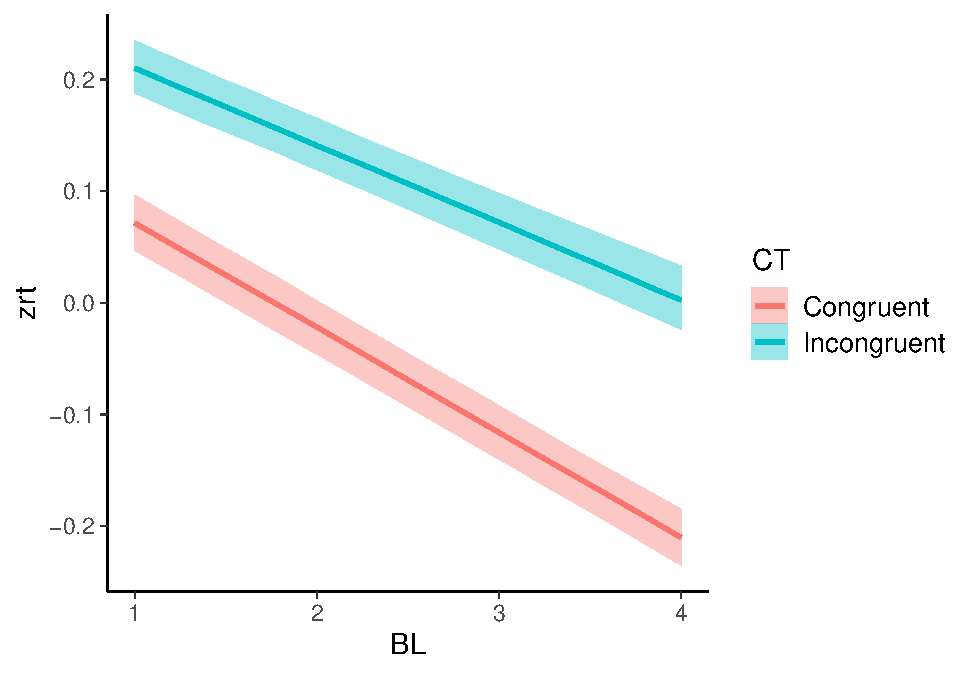
\includegraphics{20_variational_inference_files/figure-latex/Control Model with block as numeric-1.pdf}

\begin{Shaded}
\begin{Highlighting}[]
\CommentTok{\# Two{-}way interaction}
\NormalTok{c\_eff }\OtherTok{\textless{}{-}} \FunctionTok{conditional\_effects}\NormalTok{(mod\_c, }\StringTok{"BL:CT"}\NormalTok{) }
\FunctionTok{plot}\NormalTok{(c\_eff, }\AttributeTok{plot =} \ConstantTok{FALSE}\NormalTok{)[[}\DecValTok{1}\NormalTok{]] }\SpecialCharTok{+}
  \FunctionTok{theme}\NormalTok{(}\AttributeTok{legend.position =} \StringTok{"bottom"}\NormalTok{) }\SpecialCharTok{+}
  \FunctionTok{labs}\NormalTok{(}
    \AttributeTok{y =} \StringTok{"Reaction Times (standardized)"}\NormalTok{,}
    \AttributeTok{x =} \StringTok{"Block of Trials"}
\NormalTok{  )}
\end{Highlighting}
\end{Shaded}

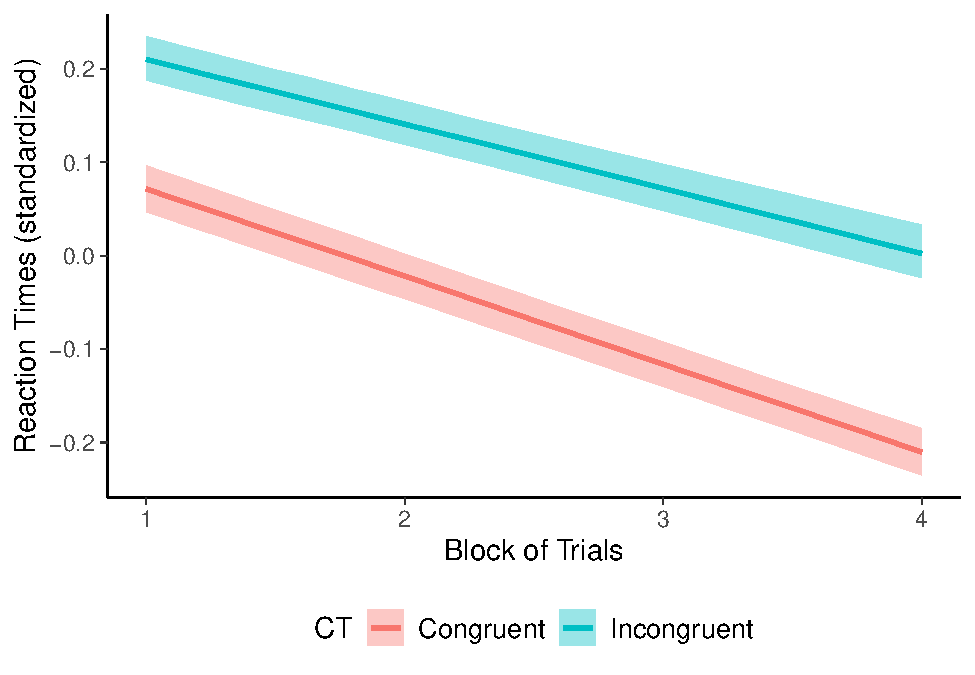
\includegraphics{20_variational_inference_files/figure-latex/Control Model with block as numeric-2.pdf}

\begin{Shaded}
\begin{Highlighting}[]
\CommentTok{\# No interaction}
\NormalTok{c4 }\OtherTok{\textless{}{-}} \FunctionTok{brm}\NormalTok{(}
  \FunctionTok{bf}\NormalTok{(zrt }\SpecialCharTok{\textasciitilde{}}\NormalTok{ CT }\SpecialCharTok{+}\NormalTok{ BL }\SpecialCharTok{+}
\NormalTok{       (}\DecValTok{1} \SpecialCharTok{+}\NormalTok{ CT }\SpecialCharTok{+}\NormalTok{ BL }\SpecialCharTok{|}\NormalTok{ subj\_id) }\SpecialCharTok{+}\NormalTok{ (}\DecValTok{1} \SpecialCharTok{|}\NormalTok{ movie\_id)}
\NormalTok{  ), }
  \AttributeTok{algorithm =} \StringTok{"meanfield"}\NormalTok{,}
  \AttributeTok{family =}\NormalTok{ brms}\SpecialCharTok{::}\FunctionTok{asym\_laplace}\NormalTok{(),}
  \AttributeTok{iter =} \DecValTok{20000}\NormalTok{, }\CommentTok{\# Increase the number of iterations}
  \AttributeTok{init =} \FloatTok{0.1}\NormalTok{,}
  \AttributeTok{data =}\NormalTok{ dc}
\NormalTok{)}
\end{Highlighting}
\end{Shaded}

\begin{verbatim}
## Compiling Stan program...
\end{verbatim}

\begin{verbatim}
## Trying to compile a simple C file
\end{verbatim}

\begin{verbatim}
## Running /Library/Frameworks/R.framework/Resources/bin/R CMD SHLIB foo.c
## using C compiler: ‘Apple clang version 14.0.3 (clang-1403.0.22.14.1)’
## using SDK: ‘MacOSX13.3.sdk’
## clang -arch arm64 -I"/Library/Frameworks/R.framework/Resources/include" -DNDEBUG   -I"/Library/Frameworks/R.framework/Versions/4.3-arm64/Resources/library/Rcpp/include/"  -I"/Library/Frameworks/R.framework/Versions/4.3-arm64/Resources/library/RcppEigen/include/"  -I"/Library/Frameworks/R.framework/Versions/4.3-arm64/Resources/library/RcppEigen/include/unsupported"  -I"/Library/Frameworks/R.framework/Versions/4.3-arm64/Resources/library/BH/include" -I"/Library/Frameworks/R.framework/Versions/4.3-arm64/Resources/library/StanHeaders/include/src/"  -I"/Library/Frameworks/R.framework/Versions/4.3-arm64/Resources/library/StanHeaders/include/"  -I"/Library/Frameworks/R.framework/Versions/4.3-arm64/Resources/library/RcppParallel/include/"  -I"/Library/Frameworks/R.framework/Versions/4.3-arm64/Resources/library/rstan/include" -DEIGEN_NO_DEBUG  -DBOOST_DISABLE_ASSERTS  -DBOOST_PENDING_INTEGER_LOG2_HPP  -DSTAN_THREADS  -DUSE_STANC3 -DSTRICT_R_HEADERS  -DBOOST_PHOENIX_NO_VARIADIC_EXPRESSION  -DBOOST_NO_AUTO_PTR  -include '/Library/Frameworks/R.framework/Versions/4.3-arm64/Resources/library/StanHeaders/include/stan/math/prim/fun/Eigen.hpp'  -D_REENTRANT -DRCPP_PARALLEL_USE_TBB=1   -I/opt/R/arm64/include    -fPIC  -falign-functions=64 -Wall -g -O2  -c foo.c -o foo.o
## In file included from <built-in>:1:
## In file included from /Library/Frameworks/R.framework/Versions/4.3-arm64/Resources/library/StanHeaders/include/stan/math/prim/fun/Eigen.hpp:22:
## In file included from /Library/Frameworks/R.framework/Versions/4.3-arm64/Resources/library/RcppEigen/include/Eigen/Dense:1:
## In file included from /Library/Frameworks/R.framework/Versions/4.3-arm64/Resources/library/RcppEigen/include/Eigen/Core:88:
## /Library/Frameworks/R.framework/Versions/4.3-arm64/Resources/library/RcppEigen/include/Eigen/src/Core/util/Macros.h:628:1: error: unknown type name 'namespace'
## namespace Eigen {
## ^
## /Library/Frameworks/R.framework/Versions/4.3-arm64/Resources/library/RcppEigen/include/Eigen/src/Core/util/Macros.h:628:16: error: expected ';' after top level declarator
## namespace Eigen {
##                ^
##                ;
## In file included from <built-in>:1:
## In file included from /Library/Frameworks/R.framework/Versions/4.3-arm64/Resources/library/StanHeaders/include/stan/math/prim/fun/Eigen.hpp:22:
## In file included from /Library/Frameworks/R.framework/Versions/4.3-arm64/Resources/library/RcppEigen/include/Eigen/Dense:1:
## /Library/Frameworks/R.framework/Versions/4.3-arm64/Resources/library/RcppEigen/include/Eigen/Core:96:10: fatal error: 'complex' file not found
## #include <complex>
##          ^~~~~~~~~
## 3 errors generated.
## make: *** [foo.o] Error 1
\end{verbatim}

\begin{verbatim}
## Start sampling
\end{verbatim}

\begin{verbatim}
## Chain 1: ------------------------------------------------------------
## Chain 1: EXPERIMENTAL ALGORITHM:
## Chain 1:   This procedure has not been thoroughly tested and may be unstable
## Chain 1:   or buggy. The interface is subject to change.
## Chain 1: ------------------------------------------------------------
## Chain 1: 
## Chain 1: 
## Chain 1: 
## Chain 1: Gradient evaluation took 0.016007 seconds
## Chain 1: 1000 transitions using 10 leapfrog steps per transition would take 160.07 seconds.
## Chain 1: Adjust your expectations accordingly!
## Chain 1: 
## Chain 1: 
## Chain 1: Begin eta adaptation.
## Chain 1: Iteration:   1 / 250 [  0%]  (Adaptation)
## Chain 1: Iteration:  50 / 250 [ 20%]  (Adaptation)
## Chain 1: Iteration: 100 / 250 [ 40%]  (Adaptation)
## Chain 1: Iteration: 150 / 250 [ 60%]  (Adaptation)
## Chain 1: Iteration: 200 / 250 [ 80%]  (Adaptation)
## Chain 1: Success! Found best value [eta = 1] earlier than expected.
## Chain 1: 
## Chain 1: Begin stochastic gradient ascent.
## Chain 1:   iter             ELBO   delta_ELBO_mean   delta_ELBO_med   notes 
## Chain 1:    100       -26378.298             1.000            1.000
## Chain 1:    200       -26012.581             0.507            1.000
## Chain 1:    300       -26083.200             0.339            0.014
## Chain 1:    400       -25528.815             0.260            0.022
## Chain 1:    500       -25169.292             0.211            0.014
## Chain 1:    600       -25122.351             0.176            0.014
## Chain 1:    700       -25148.635             0.151            0.014
## Chain 1:    800       -25078.506             0.132            0.014
## Chain 1:    900       -25048.131             0.118            0.003   MEDIAN ELBO CONVERGED
## Chain 1: 
## Chain 1: Drawing a sample of size 1000 from the approximate posterior... 
## Chain 1: COMPLETED.
\end{verbatim}

\begin{verbatim}
## Warning: Pareto k diagnostic value is 4.96. Resampling is disabled. Decreasing
## tol_rel_obj may help if variational algorithm has terminated prematurely.
## Otherwise consider using sampling instead.
\end{verbatim}

\begin{Shaded}
\begin{Highlighting}[]
\NormalTok{loo\_c4 }\OtherTok{\textless{}{-}} \FunctionTok{loo}\NormalTok{(c4)}

\CommentTok{\# Test of the interaction}
\NormalTok{comp }\OtherTok{\textless{}{-}} \FunctionTok{loo\_compare}\NormalTok{(loo\_c3, loo\_c4)}
\FunctionTok{print}\NormalTok{(comp, }\AttributeTok{digits =} \DecValTok{2}\NormalTok{)}
\end{Highlighting}
\end{Shaded}

\begin{verbatim}
##    elpd_diff se_diff
## c3   0.00      0.00 
## c4 -92.39     22.90
\end{verbatim}

\begin{Shaded}
\begin{Highlighting}[]
\FunctionTok{message}\NormalTok{(}\StringTok{"}\SpecialCharTok{\textbackslash{}n}\StringTok{20\_variational\_inference.R: done!"}\NormalTok{)}
\end{Highlighting}
\end{Shaded}

\begin{verbatim}
## 
## 20_variational_inference.R: done!
\end{verbatim}

\begin{Shaded}
\begin{Highlighting}[]
\CommentTok{\# Accuracy modeling}
\end{Highlighting}
\end{Shaded}

\begin{Shaded}
\begin{Highlighting}[]
\CommentTok{\# }\AlertTok{TODO}

\CommentTok{\# Get the accuracy split by congruency.}
\NormalTok{flanker\_accuracy }\OtherTok{\textless{}{-}} \FunctionTok{get\_flanker\_accuracy}\NormalTok{(flanker\_data, }\AttributeTok{overall =} \ConstantTok{FALSE}\NormalTok{)}
\end{Highlighting}
\end{Shaded}

\begin{verbatim}
## `summarise()` has grouped output by 'experiment', 'subj_id'. You can override
## using the `.groups` argument.
\end{verbatim}

\begin{Shaded}
\begin{Highlighting}[]
\NormalTok{flanker\_accuracy }\SpecialCharTok{|\textgreater{}} 
  \FunctionTok{group\_by}\NormalTok{(experiment, is\_congruent\_trial) }\SpecialCharTok{|\textgreater{}} 
  \FunctionTok{summarize}\NormalTok{(}
    \AttributeTok{acc =} \FunctionTok{mean}\NormalTok{(accuracy)}
\NormalTok{  )}
\end{Highlighting}
\end{Shaded}

\begin{verbatim}
## `summarise()` has grouped output by 'experiment'. You can override using the
## `.groups` argument.
\end{verbatim}

\begin{verbatim}
## # A tibble: 4 x 3
## # Groups:   experiment [2]
##   experiment is_congruent_trial   acc
##   <fct>      <chr>              <dbl>
## 1 control    Congruent          0.967
## 2 control    Incongruent        0.954
## 3 surprise   Congruent          0.963
## 4 surprise   Incongruent        0.961
\end{verbatim}

\begin{Shaded}
\begin{Highlighting}[]
\CommentTok{\# eof {-}{-}{-}{-}}
\end{Highlighting}
\end{Shaded}


\end{document}
